\documentclass{article}

% Language setting
\usepackage[english]{babel}
\usepackage{float}        % for [H]
\usepackage{pdflscape}    % rotates a single page to landscape (PDF rotation)

\usepackage[letterpaper,top=2cm,bottom=2cm,left=3cm,right=3cm,marginparwidth=1.75cm]{geometry}

% Useful packages
\usepackage{amsmath}
\usepackage{amsfonts}
\usepackage{amssymb}
\usepackage{microtype}
\usepackage{graphicx}
\usepackage{tabularx}
\usepackage{subcaption}
\usepackage{siunitx}
\usepackage{booktabs}
\usepackage[table]{xcolor}
\usepackage{array}
\usepackage{enumitem}
\usepackage{algorithm}
\usepackage{algpseudocode}
\usepackage[colorlinks=true, allcolors=blue]{hyperref}

\hypersetup{
    colorlinks=true,
    linkcolor=blue,
    citecolor=blue,
    urlcolor=blue
}

\newcommand{\code}[1]{\texttt{#1}}
\newcommand{\hz}[1]{{\color{blue} [#1 -HZ]}}
\newcommand{\tz}[1]{{\color{red} [#1 -TZ]}}

% Placeholder command: red, bold, bracketed. Used wherever a figure,
% photo, table of results, or missing detail still has to be inserted.
\newcommand{\highlight}[1]{{\color{red}\textbf{[TO ADD: #1]}}}

% Report-wide shorthands
\newcommand{\Tone}{T_1}
\newcommand{\Ttwo}{T_2}
\newcommand{\Tproc}{T_{\mathrm{proc},1}}
\newcommand{\Lsub}{L_{\mathrm{subCH}}}
\newcommand{\Prsvp}{P_{\mathrm{rsvp}}}
\newcommand{\pass}{PASS}
\newcommand{\fail}{\textbf{FAIL}}

\begin{document}

{\center

\vfill
\IfFileExists{figures/wici.jpg}{
\includegraphics[width=3in]{figures/wici.jpg}}{\highlight{figures/wici.jpg}}\\[0cm]
\vfill

{\large
5G Sidelink Evaluation: Simulation Study Report\\
\hspace*{0.15cm} (October 2026)
}

\vspace*{0.3in}

{\Large \textbf{\\5G NR Sidelink Mode 2 for Agricultural Machine-to-Machine
Communication: MAC Procedures, Link-Level and System-Level Evaluation
}}

\vspace*{0.2in}
{\normalsize
\vspace*{0.1in}
Md Saidur Rahman, Tianyi Zhang, Hongwei Zhang \\
Center for Wireless, Communities and Innovation (WiCI) \\
Iowa State University  \\
\texttt{\{shaown,tianyiz,hongwei\}@iastate.edu }\\

\vspace*{0.2in}

Dino Joseph Mycle, Long Hoang, Mike Kool, Robert Kinyanjui\\
John Deere\\
\texttt{\{MycleDinoJoseph,HoangLong,KoolMichaelA,KinyanjuiRobertK\}@johndeere.com}

\vspace*{4.2in}

}

}

\newpage

\pagenumbering{roman}
\tableofcontents
\listoffigures
\listoftables

\newpage

\clearpage
\pagenumbering{arabic}
\setcounter{page}{1}

%==========================================================================
\section*{Executive Summary}
\addcontentsline{toc}{section}{Executive Summary}

This report evaluates 3GPP Release~16 NR sidelink Mode~2 for broadcast
machine-to-machine communication in an open agricultural field, using a
clause-cited MATLAB implementation of the sidelink stack
(\code{nrSidelink}). The study is built in three steps, each resting on
the one before.

\paragraph{Part A: MAC procedures.} We describe what the specification
promises and how a UE senses, excludes and selects resources:
sensing-based semi-persistent scheduling (SPS) for periodic traffic and
one-shot selection for event traffic. With $\Tone = \Tproc = 5$ slots,
$\Ttwo = \mathrm{PDB} - 3$ slots, and a latency that counts the
transmission slot and two receive slots, no packet can be delivered
sooner than 4~ms or later than its packet delay budget (PDB). On an
empty channel the implementation keeps both bounds for every one of
5000 packets across the five broadcast PQIs.

\paragraph{Part B: one link, real PHY.} Range, throughput and latency of
a single link are measured over the full PSCCH/PSSCH chains with TDL-D
fading at 0--30~mph. With TR~38.901 RMa line-of-sight path loss, antennas
at 3~m on the machinery, 3~dBi per antenna and a 9~dB noise figure
(TR~37.885 \cite{ref:37885}), MCS~5 reaches 1500~m on its first
transmission, MCS~1--3 reach 1.7--1.9~km, MCS~11 carries 14.3~Mbit/s to
about 1.15~km, and MCS~27 carries 25--50~Mbit/s only inside about 200~m.
Speed up to 30~mph barely matters except for MCS~27.

\paragraph{Part C: many UEs in a field.} UEs are dropped as a Poisson
point process in a 1~km~$\times$~1~km field at densities from 5 to
100~UE/km$^2$. Every UE carries all five broadcast PQIs (48~kbit/s), and
every flow is judged against its own packet error rate. The 90\% flows
hold their targets to about 48--72~UE/km$^2$, the 99\% sensor-sharing
flow to about 32~UE/km$^2$, and the 99.99\% lane-change flow at no
density. Broadcast throughput, counted at the receivers, reaches every
intended receiver with at least 98.8\% efficiency up to 30~UE/km$^2$
and falls to 80\% at 100~UE/km$^2$. Latency does not grow with density:
contention costs packets, not time. Every loss is a collision or half
duplex; the radio link is never the limit inside 500~m.

%==========================================================================
\section{Introduction}
\label{sec:intro}

\subsection{How to Read this Report}

\begin{enumerate}[nosep]
  \item \textbf{Part A (Section~\ref{sec:partA}) -- MAC procedures.}
  What the specification promises, and how a UE senses, excludes and
  selects resources. No radio channel is needed to explain this.
  \item \textbf{Part B (Section~\ref{sec:partB}) -- one link, real PHY.}
  Range, throughput and latency of a single link for MCS 5, 6, 11 and 27
  against distance and speed. The physical layer is simulated, not
  abstracted.
  \item \textbf{Part C (Section~\ref{sec:partC}) -- many UEs in a field.}
  A 1~km~$\times$~1~km deployment at several densities, with the traffic
  flows stated first and every flow judged against its own packet error
  rate.
\end{enumerate}

\subsection{The Setup}
\label{sec:setup}

\begin{table}[H]
\centering
\caption{Operating point used throughout the study.}
\label{tab:setup}
\small
\begin{tabularx}{\textwidth}{l X}
\toprule
\textbf{Item} & \textbf{Value} \\
\midrule
Channel & 20~MHz at 5.9~GHz, 30~kHz subcarrier spacing ($\mu = 1$), 0.5~ms slots \\
Resource pool & 5 sub-channels $\times$ 10 PRB = 50 PRB \\
Transmit power & 23~dBm \\
Propagation & TR~38.901 RMa, line of sight (an open agricultural field) \cite{ref:38901}; antennas 3~m above ground at both ends (machinery cab roof) \\
Antennas & 3~dBi per antenna, 6~dB combined (transmitter + receiver) \\
Receiver & noise figure 9~dB, the vehicle/pedestrian UE value of 3GPP TR~37.885 V15.3.0, Table~6.1.1-1 \cite{ref:37885} \\
Fading & TDL-D (line of sight with multipath), 100~ns delay spread, at 0 / 10 / 20 / 30~mph \\
Selection window & $\Tone = 5$ slots (2.5~ms), the largest TS~38.214 allows at $\mu = 1$ \cite{ref:38214}; $\Ttwo = \mathrm{PDB} - 3$ slots \\
Latency pipeline & the transport block is built during $\Tone$; then 1 transmission slot and 2 slots to receive it \\
Traffic classes & the five broadcast PQIs of TS~23.287 Table~5.4.4-1: 55, 56, 57, 58, 59 \cite{ref:23287} \\
\bottomrule
\end{tabularx}
\end{table}

\paragraph{What a latency is here.} A packet arrives in slot $n$ and is
transmitted in slot $n + k$. The transport block (TB) is generated
during $\Tone$: that preparation is what $\Tproc$ is for. The packet is
delivered at slot $n + k + 3$:
\begin{itemize}[nosep]
  \item \textbf{1 slot} is the transmission slot itself, while the TB is on the air;
  \item \textbf{2 slots} are for the receiver to demodulate, decode and pass it up.
\end{itemize}
Every latency in this report includes those three slots. With $k$
drawn uniformly in $[\Tone, \Ttwo]$:
\begin{equation}
\label{eq:latency}
D = k + 3 \text{ slots}, \qquad
\bar{D} = \frac{\Tone + \Ttwo}{2} + 3 \text{ slots}, \qquad
\Ttwo = \mathrm{PDB} - 3 \text{ slots}.
\end{equation}

\paragraph{$\Tone$ and $\Ttwo$.} The UE may place its transmission
anywhere in $[n + \Tone, n + \Ttwo]$.
\begin{itemize}[nosep]
  \item $\Tone$ must be at least the processing time $\Tproc$
  (TS~38.214 Table~8.1.4-2: 5 slots at $\mu = 1$) \cite{ref:38214}, and
  we take exactly that.
  \item $\Ttwo$ may not exceed the remaining delay budget. Because the
  transmission slot and the two reception slots must all fit inside the
  PDB, the last allowed slot is $\Ttwo = \mathrm{PDB} - 3$ slots: the
  transmission ends two slots before the deadline and the receiver
  finishes exactly at it. For PDB~10~ms (20 slots), $\Ttwo = 17$ slots.
  \item No transport block may carry a packet younger than $\Tproc$, on
  any grant. Without this rule, a packet arriving while the UE already
  holds an SPS grant could go out in its own arrival slot.
\end{itemize}
So \textbf{no packet can be delivered sooner than $\Tone + 3$ slots =
4~ms, nor later than its PDB.}

\paragraph{Which PQIs.} TS~23.287 Table~5.4.4-1 (V19.0.0) defines ten
PQIs \cite{ref:23287}. Its NOTE~1 states that \emph{``GBR and Delay
Critical GBR PQIs can only be used for unicast PC5 communications''},
which leaves broadcast with the five Non-GBR rows of
Table~\ref{tab:pqi}. A flow \emph{passes} when at least $1 -
\mathrm{PER}$ of its packets arrive within the PDB at each intended
receiver.

\begin{table}[H]
\centering
\caption{The broadcast (Non-GBR) PQIs of TS~23.287 Table~5.4.4-1 \cite{ref:23287}.}
\label{tab:pqi}
\small
\begin{tabularx}{\textwidth}{c c c c c X}
\toprule
\textbf{PQI} & \textbf{Priority} & \textbf{PDB} & \textbf{PER} & \textbf{Target} & \textbf{Example service} \\
\midrule
55 & 3 & 10~ms  & $10^{-4}$ & 99.99\% & cooperative lane change, higher degree of automation \\
56 & 6 & 20~ms  & $10^{-1}$ & 90\%    & platooning informative exchange; information sharing with an RSU \\
57 & 5 & 25~ms  & $10^{-1}$ & 90\%    & cooperative lane change, lower degree of automation \\
58 & 4 & 100~ms & $10^{-2}$ & 99\%    & sensor information sharing, lower degree of automation \\
59 & 6 & 500~ms & $10^{-1}$ & 90\%    & platooning, reporting to an RSU \\
\bottomrule
\end{tabularx}
\end{table}

%==========================================================================
\newpage
\section{Part A: How Mode 2 Picks Resources}
\label{sec:partA}

\subsection{What the Specification Promises}
\label{sec:promise}

\begin{figure}[H]
  \centering
  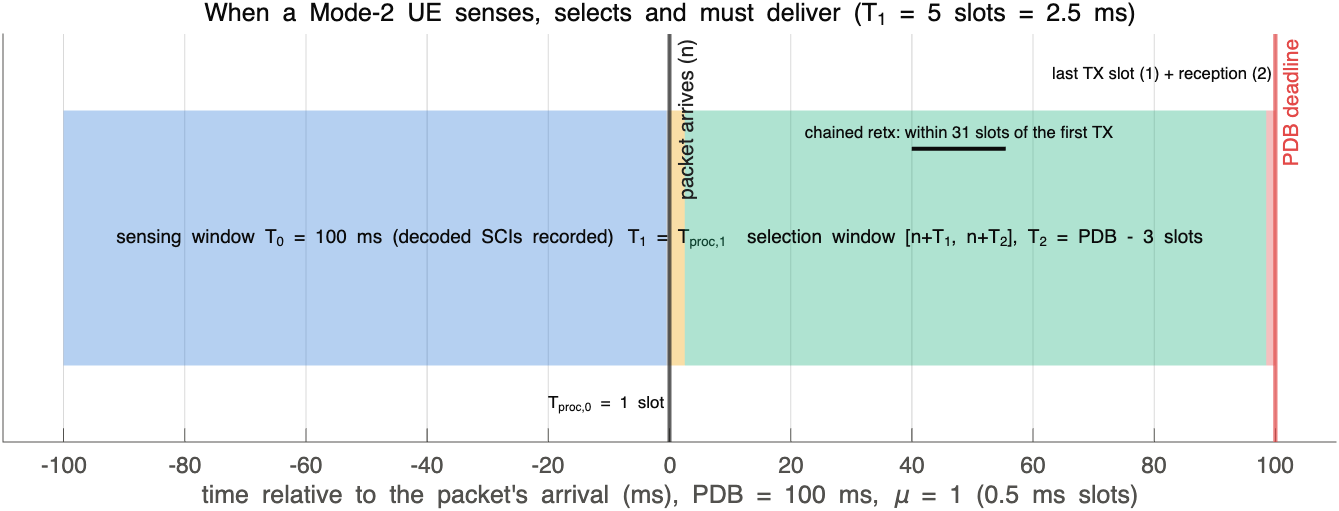
\includegraphics[width=\textwidth]{figures/A1_window_timeline.png}
  \caption{When a UE senses, selects and must deliver.}
  \label{fig:A1}
\end{figure}

How to read Fig.~\ref{fig:A1}:
\begin{itemize}[nosep]
  \item Time runs left to right around the packet's arrival at $n$.
  \item For the past 100~ms (the sensing window, \code{sl-SensingWindow})
  the UE has been decoding its neighbours' control messages.
  \item It needs $\Tproc = 2.5$~ms to prepare, then may transmit
  anywhere in the selection window.
  \item The last three slots before the PDB are the last transmission
  slot and the two slots the receiver needs.
  \item A blind retransmission must follow within 31 slots of the first
  transmission, because that is all the SCI's TRIV field can announce
  (TS~38.214 \S8.1.5) \cite{ref:38214}.
\end{itemize}

The delivered latency is therefore bounded on both sides:
\begin{itemize}[nosep]
  \item \textbf{minimum} $= \Tone + 3$ slots $= 4$~ms, whatever the PDB;
  \item \textbf{maximum} $= \Ttwo + 3$ slots $=$ the PDB itself;
  \item \textbf{mean} $= (\Tone + \Ttwo)/2 + 3$ slots when the UE draws
  uniformly in the window, as Mode~2 does. For PQI~55:
  $(5 + 17)/2 + 3 = 14$ slots $= 7$~ms.
\end{itemize}

\begin{figure}[H]
  \centering
  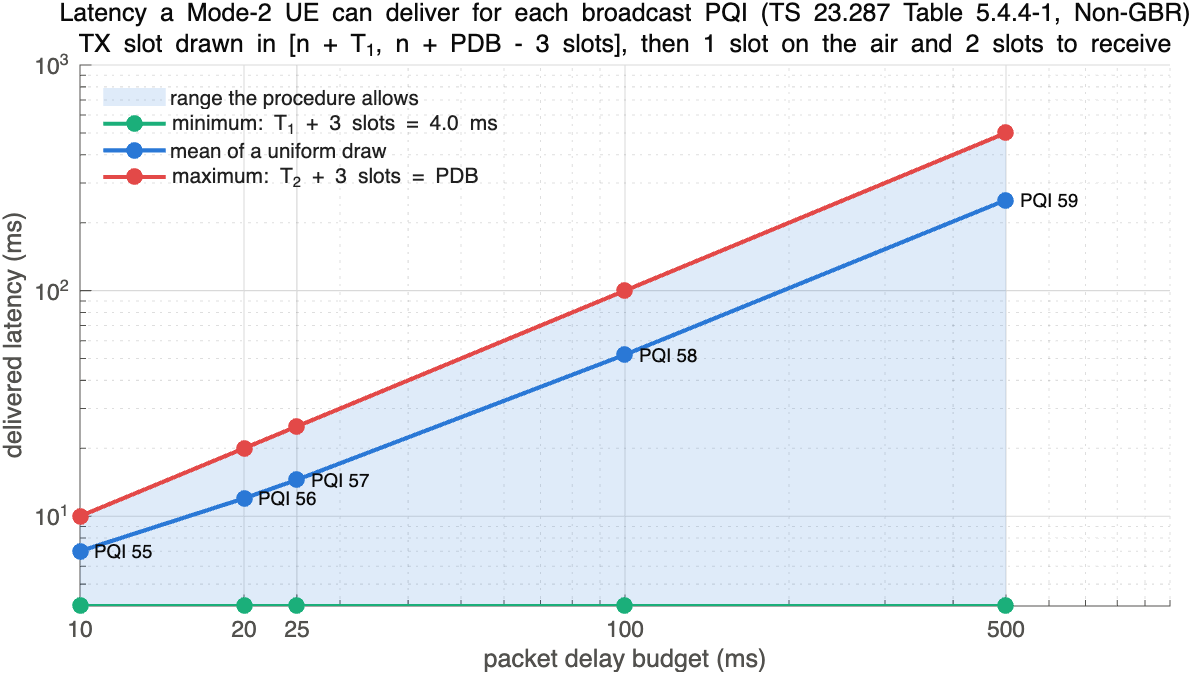
\includegraphics[width=0.85\textwidth]{figures/A2_latency_bounds.png}
  \caption{The latency each broadcast PQI allows. The band is everything
  the procedure permits; the middle line is where a uniform draw lands
  on average.}
  \label{fig:A2}
\end{figure}

\begin{table}[H]
\centering
\caption{Latency bounds per broadcast PQI.}
\label{tab:bounds}
\small
\begin{tabular}{c c c c c c}
\toprule
\textbf{PQI} & \textbf{PDB} & $\Ttwo$ & \textbf{Minimum} & \textbf{Mean (uniform draw)} & \textbf{Maximum} \\
\midrule
55 & 10~ms  & 17 slots  & 4~ms & 7~ms    & 10~ms \\
56 & 20~ms  & 37 slots  & 4~ms & 12~ms   & 20~ms \\
57 & 25~ms  & 47 slots  & 4~ms & 14.5~ms & 25~ms \\
58 & 100~ms & 197 slots & 4~ms & 52~ms   & 100~ms \\
59 & 500~ms & 997 slots & 4~ms & 252~ms  & 500~ms \\
\bottomrule
\end{tabular}
\end{table}

\textbf{The key point for everything that follows:} in Mode~2, latency is
set by \emph{where in the window the UE draws its resource}, not by the
radio. A PQI~58 message waits about 52~ms on average even on an empty
channel. Delivering earlier means a shorter window, and a shorter window
means fewer candidates to choose from.

\subsection{Sensing: What a UE Hears}
\label{sec:sensed}

\begin{figure}[H]
  \centering
  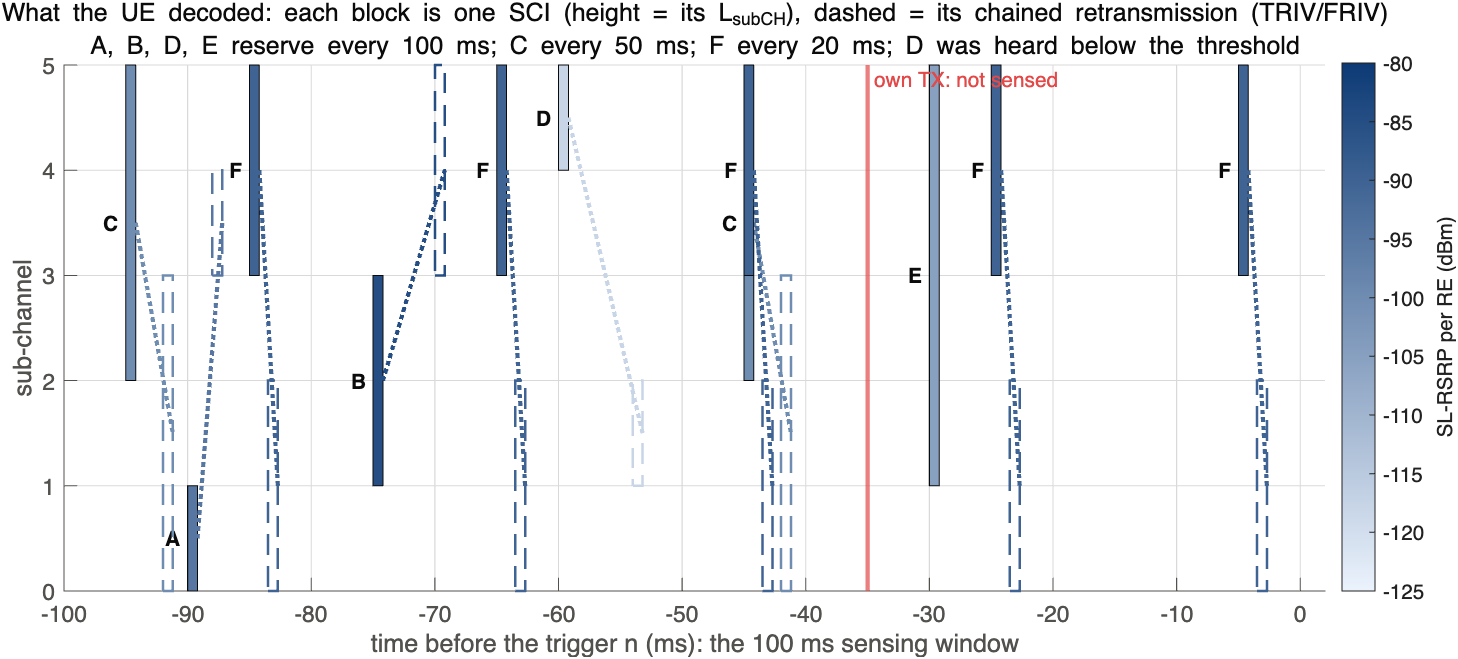
\includegraphics[width=\textwidth]{figures/A3_sensed_scis.png}
  \caption{One UE's sensing window: the SCI-1A messages it decoded.}
  \label{fig:A3}
\end{figure}

How to read Fig.~\ref{fig:A3}: each solid block is one control message
(SCI-1A) the UE decoded \cite{ref:38212}. Its horizontal position is the
slot it was heard in, its vertical span the sub-channels it occupied
(its $\Lsub$: from 1 to 4 here), and its shade the received power per
resource element (SL-RSRP) \cite{ref:38215}. The dashed box joined to it
is the chained retransmission the same SCI announced (TRIV gives the slot
offset, FRIV the sub-channel). The red line is a slot the UE was itself
transmitting in, so it heard nothing there (half duplex). The six
neighbours of Table~\ref{tab:nbrs} were chosen to show every case.

\begin{table}[H]
\centering
\caption{The six neighbours in the sensing example.}
\label{tab:nbrs}
\small
\begin{tabular}{c c c c l}
\toprule
\textbf{Neighbour} & \textbf{Width $\Lsub$} & \textbf{Reserves every} & \textbf{RSRP} & \textbf{Note} \\
\midrule
A & 1 & 100~ms & $-95$~dBm  & \\
B & 2 & 100~ms & $-85$~dBm  & \\
C & 3 & 50~ms  & $-100$~dBm & heard twice in the window \\
D & 1 & 100~ms & $-118$~dBm & \textbf{below} the $-110$~dBm threshold \\
E & 4 & 100~ms & $-105$~dBm & no chained retransmission \\
F & 2 & 20~ms  & $-90$~dBm  & heard five times \\
\bottomrule
\end{tabular}
\end{table}

Every SCI carries the sender's \textbf{reservation period}, so a receiver
knows not only where the sender was but where it will be next.

\subsection{From Sensing to a Candidate Set}
\label{sec:candidates}

When a packet arrives, the UE lists every possible resource in its
selection window: each slot $\times$ each starting sub-channel that fits
its own width (here $\Lsub = 2$). That is the candidate set,
$M_{\mathrm{total}} = 772$ resources for a 100~ms window. It then removes
every candidate that would overlap a neighbour's \textbf{projected}
reservation heard above the RSRP threshold (TS~38.214 \S8.1.4)
\cite{ref:38214}.

\begin{figure}[H]
  \centering
  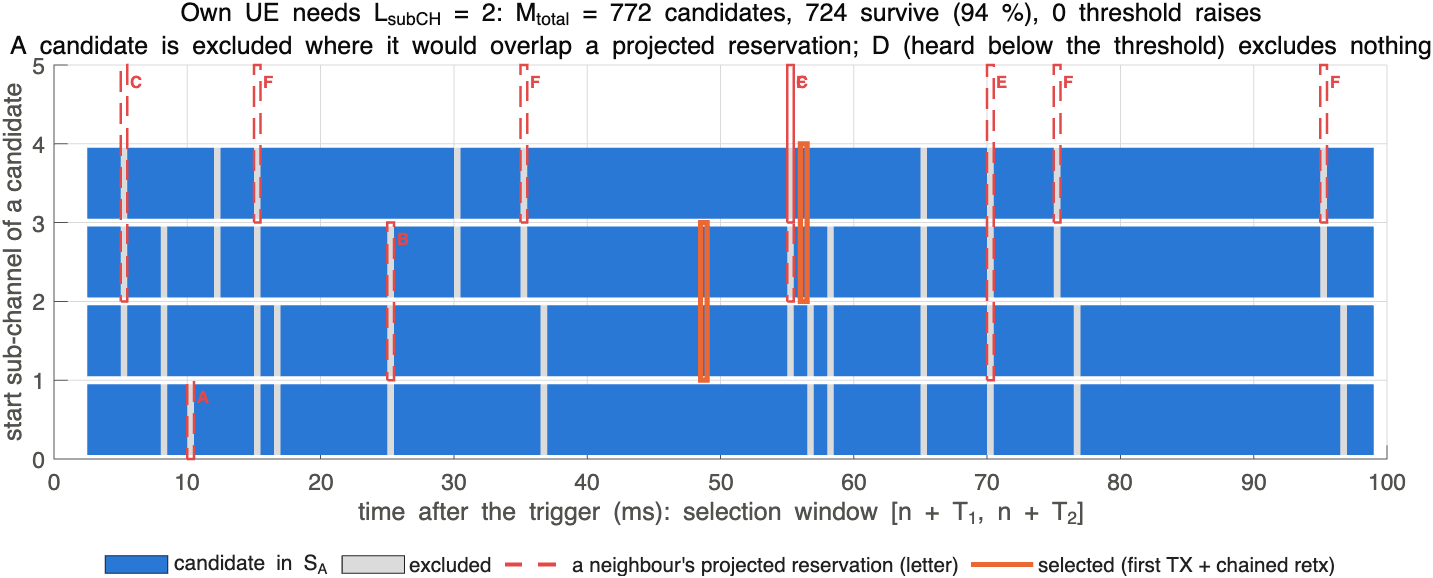
\includegraphics[width=\textwidth]{figures/A4_exclusion.png}
  \caption{Exclusion in the selection window.}
  \label{fig:A4}
\end{figure}

How to read Fig.~\ref{fig:A4}: blue cells survive, grey cells are
excluded, dashed red outlines are the neighbours' projected reservations
(letters as in Fig.~\ref{fig:A3}). F, which reserves every 20~ms, blocks
a column every 20~ms; D, heard below the threshold, blocks nothing. The
unlabelled grey slivers are projected chained retransmissions and the
slots the UE could not sense (the specification assumes the worst for
those). The UE then draws its resource at random from the survivors
(orange): here 724 of 772 survive (94\%).

\begin{figure}[H]
  \centering
  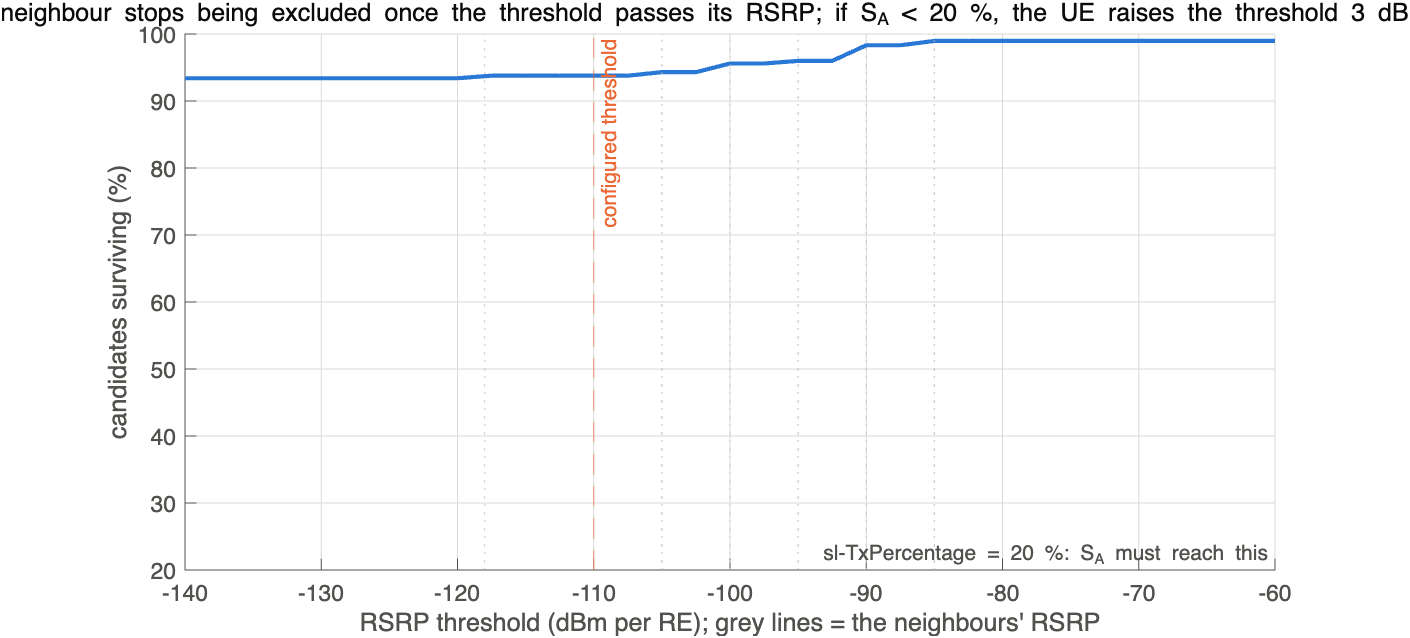
\includegraphics[width=\textwidth]{figures/A5_threshold.png}
  \caption{The RSRP threshold and the escalation rule.}
  \label{fig:A5}
\end{figure}

If fewer than \code{sl-TxPercentage} = 20\% of candidates survive, the UE
raises the RSRP threshold by 3~dB and tries again (Fig.~\ref{fig:A5}).
Each neighbour stops being excluded once the threshold passes its RSRP
(grey lines). In a crowded channel this is how a UE still finds a
resource: by accepting overlap with distant, weak neighbours.

\subsection{Periodic Traffic: Sensing-Based Semi-Persistent Scheduling}
\label{sec:sps}

For a periodic message, the UE keeps the selected resource and reuses it
every reservation period, announcing each next use in its SCI.

\begin{figure}[H]
  \centering
  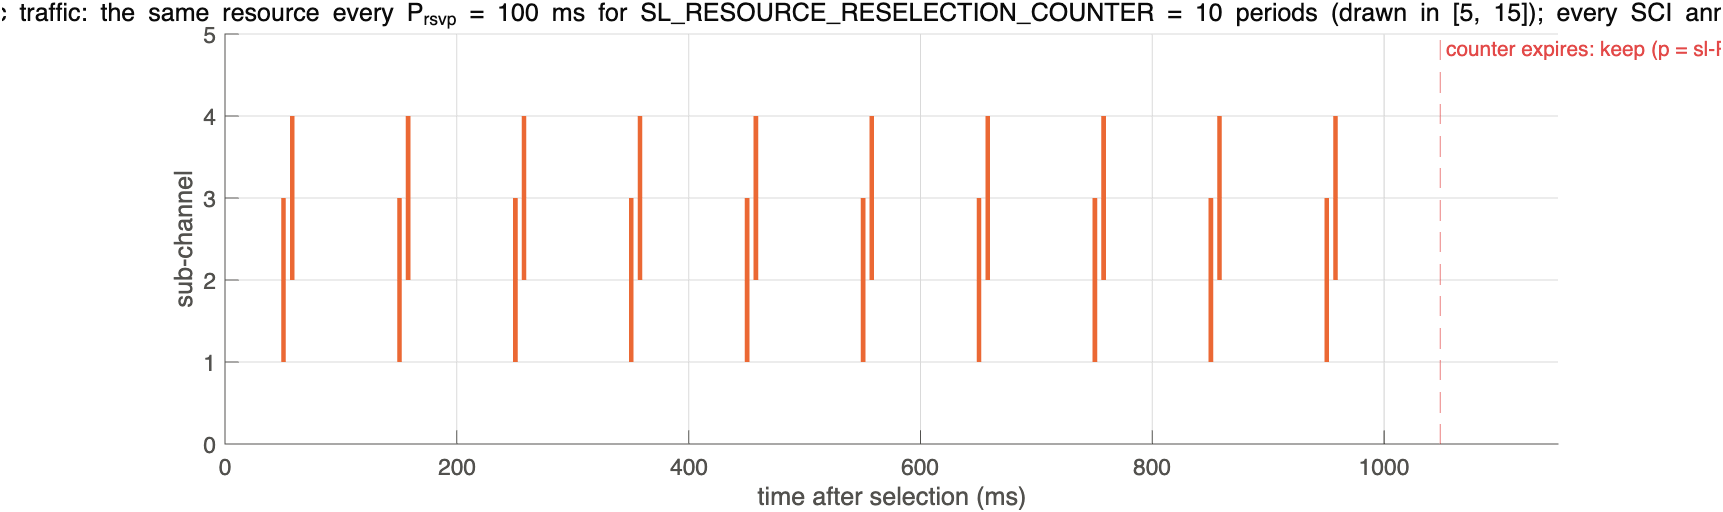
\includegraphics[width=\textwidth]{figures/A6_sps_reservation.png}
  \caption{One SPS reservation.}
  \label{fig:A6}
\end{figure}

The resource (and its chained retransmission) repeats every
$\Prsvp = 100$~ms for a random number of periods (TS~38.321
\S5.22.1.1: 5--15 periods at 100~ms) \cite{ref:38321}. When the counter
expires, the UE keeps the resource with probability
\code{sl-ProbResourceKeep} (0.4 here) or selects a new one.

\begin{figure}[H]
  \centering
  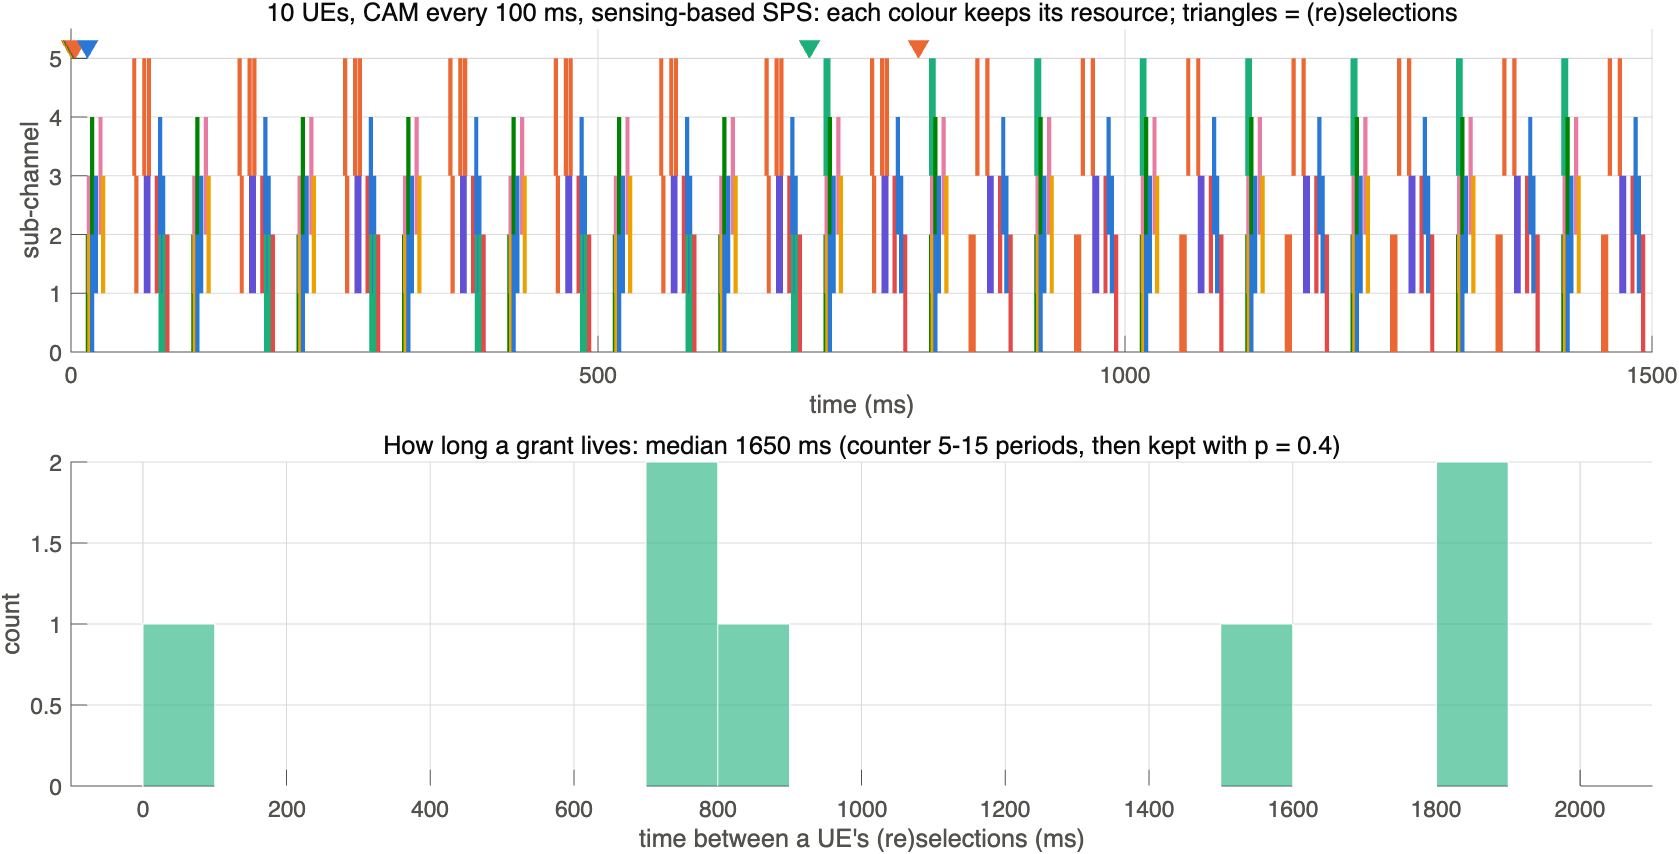
\includegraphics[width=\textwidth]{figures/A7_sps_in_action.png}
  \caption{SPS in a running simulation: 10 UEs sending a PQI~58 message
  every 100~ms.}
  \label{fig:A7}
\end{figure}

How to read Fig.~\ref{fig:A7}: each colour is one UE; the same colour
returning to the same sub-channels every 100~ms is SPS at work, and
triangles mark (re)selections. A grant lives about 1.65~s (median), so
neighbours have more than a second to learn and avoid it. That is why
sensing works well for periodic traffic: none of the transmissions in
this run collided.

\subsection{Event Traffic: One-Shot Selection}
\label{sec:event}

An event message (a cooperative lane change, PQI~55 or~57) arrives at a
random time and needs no reservation for later. The UE performs a
one-shot selection with no reservation period ($\Prsvp = 0$) in the same
window $[n + \Tone, n + \mathrm{PDB} - 3]$, using the same sensing
history.

\begin{figure}[H]
  \centering
  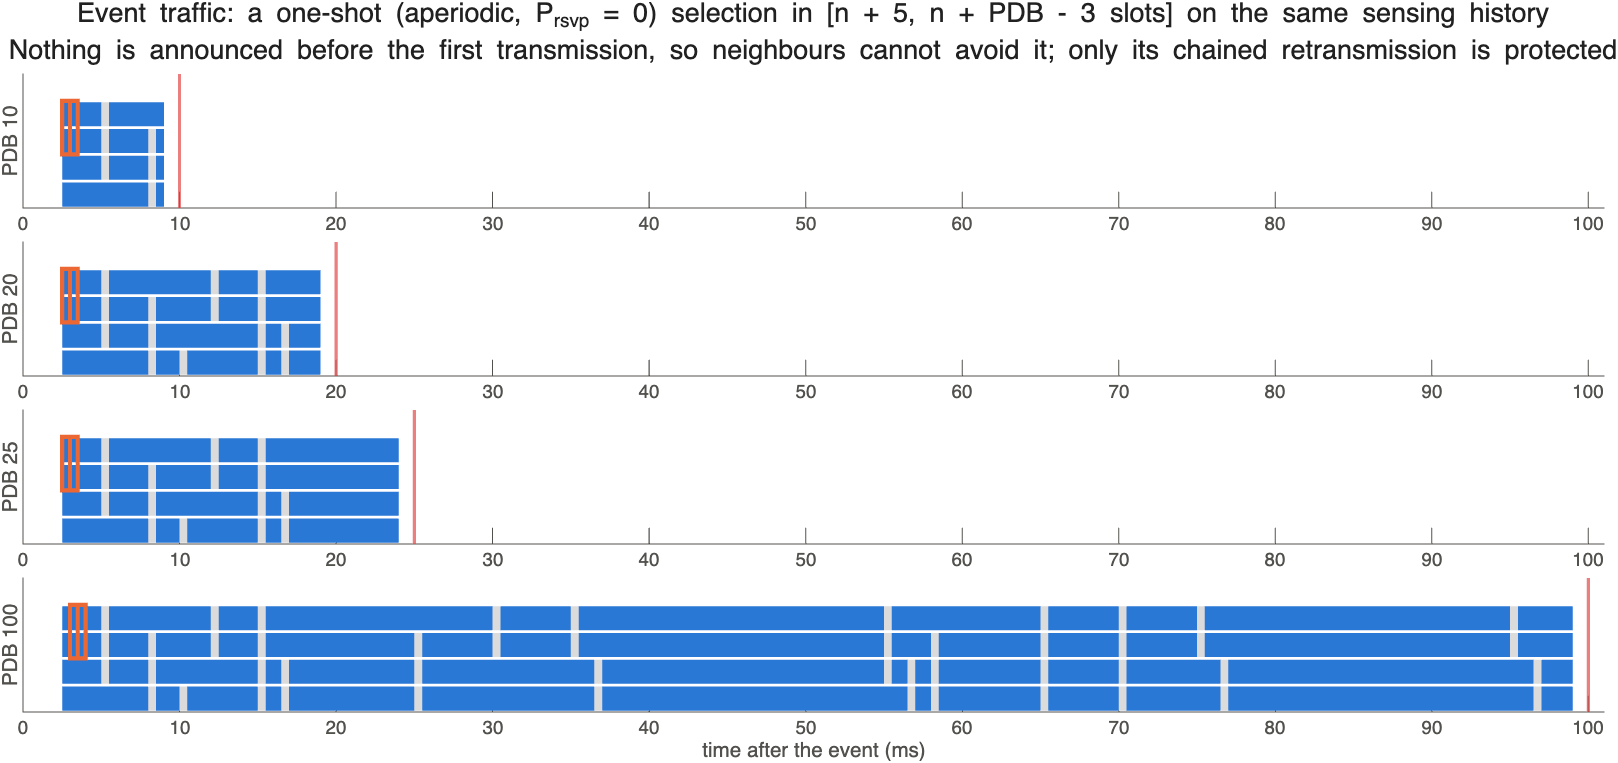
\includegraphics[width=\textwidth]{figures/A8_event_selection.png}
  \caption{Event selection for the PDBs of PQI 55, 56, 57 and 58 (10, 20,
  25, 100~ms).}
  \label{fig:A8}
\end{figure}

The window shrinks with the PDB: for PDB~10~ms only 52 candidates exist
(46 survive), against 772 for 100~ms (Table~\ref{tab:event}).

\begin{table}[H]
\centering
\caption{One-shot event selection per PDB.}
\label{tab:event}
\small
\begin{tabular}{l c c c c}
\toprule
\textbf{PDB} & \textbf{Transmission window} & $M_{\mathrm{total}}$ & \textbf{Surviving} & \textbf{Latency min / mean / max} \\
\midrule
10~ms (PQI 55)  & 2.5--8.5~ms  & 52  & 46  & 4 / 7 / 10~ms \\
20~ms (PQI 56)  & 2.5--18.5~ms & 132 & 117 & 4 / 12 / 20~ms \\
25~ms (PQI 57)  & 2.5--23.5~ms & 172 & 157 & 4 / 14.5 / 25~ms \\
100~ms (PQI 58) & 2.5--98.5~ms & 772 & 724 & 4 / 52 / 100~ms \\
\bottomrule
\end{tabular}
\end{table}

\textbf{The cost of a one-shot selection:} nothing announces the first
transmission before it happens, so neighbours cannot avoid it. Only its
chained retransmission is protected (the first SCI announces it). Two
event messages from nearby UEs can therefore land on the same resource,
which SPS largely avoids.

\subsection{Every Packet within its PDB, on an Empty Channel}
\label{sec:perpacket}

The bounds above are what the procedure allows. This section checks that
the implementation keeps them, packet by packet. One UE sends 1000
packets of each broadcast PQI to one receiver 100~m away, with nothing
else on the channel. The full system-level MAC runs: sensing, SPS,
reselection when a grant cannot meet the PDB, and one blind
retransmission. Each PQI keeps the traffic shape of its service:
\begin{itemize}[nosep]
  \item the lane-change PQIs (55, 57) are events, arriving as a Poisson
  process with a 100~ms mean;
  \item PQIs 56 and 58 are periodic every 100~ms; PQI~59 is periodic
  every 500~ms.
\end{itemize}

\begin{figure}[H]
  \centering
  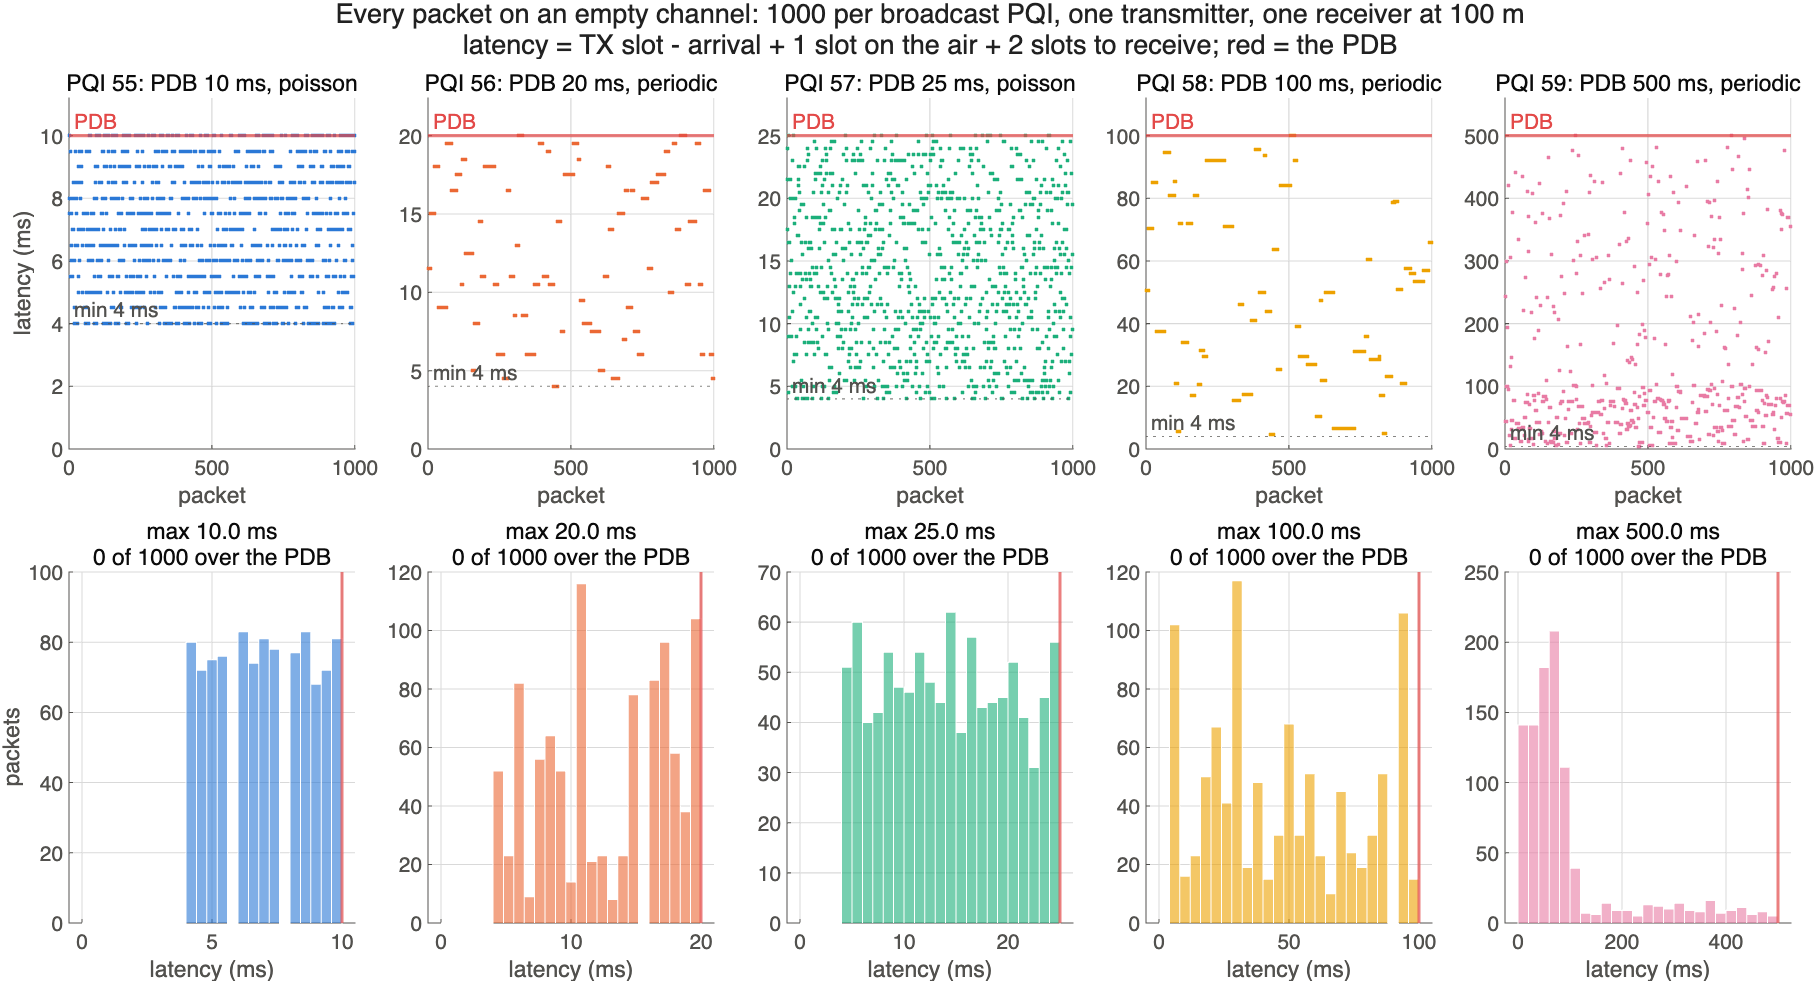
\includegraphics[width=\textwidth]{figures/A9_per_packet_latency.png}
  \caption{The latency of every packet, 1000 per broadcast PQI. Top: one
  dot per packet in order of arrival (red: PDB; dotted: the 4~ms floor).
  Bottom: the same latencies as a histogram.}
  \label{fig:A9}
\end{figure}

\begin{table}[H]
\centering
\caption{Per-packet latency on an empty channel.}
\label{tab:perpacket}
\footnotesize\setlength{\tabcolsep}{3.5pt}
\begin{tabular}{c c l c c c c c}
\toprule
\textbf{PQI} & \textbf{PDB} & \textbf{Traffic} & \textbf{Packets} & \textbf{Min} & \textbf{Mean} & \textbf{Max} & \textbf{Over the PDB} \\
\midrule
55 & 10~ms  & events, mean 100~ms & 1000 & 4.0~ms & 7.0~ms  & 10.0~ms  & \textbf{0} \\
56 & 20~ms  & every 100~ms        & 1000 & 4.0~ms & 12.6~ms & 20.0~ms  & \textbf{0} \\
57 & 25~ms  & events, mean 100~ms & 1000 & 4.0~ms & 14.0~ms & 25.0~ms  & \textbf{0} \\
58 & 100~ms & every 100~ms        & 1000 & 4.5~ms & 47.0~ms & 100.0~ms & \textbf{0} \\
59 & 500~ms & every 500~ms        & 1000 & 4.5~ms & 97.8~ms & 500.0~ms & \textbf{0} \\
\bottomrule
\end{tabular}
\end{table}

\textbf{No packet of any PQI misses its PDB, and none arrives sooner than
4~ms.} The maximum equals the PDB exactly, as the window allows. Three
patterns are worth reading in Fig.~\ref{fig:A9}:
\begin{itemize}[nosep]
  \item \textbf{Events (55, 57) spread uniformly} between 4~ms and the
  PDB: every event makes a fresh draw.
  \item \textbf{Periodic traffic (56, 58) forms horizontal runs.} A
  selected resource is reused every period, so consecutive packets see
  the same latency until the grant is reselected.
  \item \textbf{PQI~59} is mostly delivered within about 100~ms, well
  inside its budget. It is periodic at 500~ms but reserves every 100~ms,
  so it usually finds a reserved slot soon after arriving.
\end{itemize}

\paragraph{Two simulator faults found and fixed by this check.}
\begin{enumerate}[nosep]
  \item A packet arriving onto an existing SPS grant could be sent in
  its own arrival slot, giving 1.5~ms latencies below the 4~ms floor.
  Packets younger than $\Tproc$ are now held back.
  \item When two lane-change events arrived 2--4 slots apart, the grant
  chosen for the first had no room for the second. After the first went
  out, too little budget was left to reselect, so the second expired
  unsent: 3 of 1000 PQI~55 packets. The MAC now reselects as soon as the
  pending data no longer fits.
\end{enumerate}

\subsection{Part A Summary}

Mode~2 lets a UE deliver a packet no sooner than 4~ms after it arrives
($\Tone = 2.5$~ms of preparation, then 1 slot on the air and 2 slots to
receive) and no later than its PDB. A uniform draw lands in the middle on
average. On an empty channel the implementation keeps both bounds for
every one of 5000 packets across the five broadcast PQIs. Sensing
protects a transmission only when it was announced in advance: always
for SPS (every period announces the next), never for the first
transmission of an event. Everything in Parts B and C is this procedure
running over a real radio link.

%==========================================================================
\newpage
\section{Part B: One Link, Real PHY}
\label{sec:partB}

Every number here comes from the \textbf{link-level simulator}: the
normative PSCCH/PSSCH transmit chains \cite{ref:38211,ref:38212}, a real
OFDM waveform, a TDL-D fading channel with an independent realisation
for every transport block, channel estimation from the DM-RS,
equalisation, LDPC decoding with HARQ soft combining, and the CRC check.
Nothing is approximated by a formula. The only inputs are distance
(through the link budget) and speed (through the fading).

\subsection{The Link Budget}
\label{sec:budget}

The received SNR per resource element over 50 PRB is
\begin{equation}
\label{eq:snr}
\mathrm{SNR}(d) = 23~\text{dBm} + G - PL_{\mathrm{RMa}}(d) - 10\log_{10}(12 \times 50) - N_{\mathrm{RE}},
\end{equation}
with $N_{\mathrm{RE}} = -174~\text{dBm/Hz} + 10\log_{10}(30~\text{kHz}) + 9~\text{dB} = -120.2$~dBm.
Each term and its source are listed in Table~\ref{tab:budget}.

\begin{table}[H]
\centering
\caption{Link budget terms.}
\label{tab:budget}
\small
\begin{tabularx}{\textwidth}{l l X}
\toprule
\textbf{Term} & \textbf{Value} & \textbf{Source} \\
\midrule
Transmit power & 23~dBm & $P_{\mathrm{CMAX}}$ of the operating point \\
Path loss $PL_{\mathrm{RMa}}$ & Rural Macro, LOS, 5.9~GHz & 3GPP TR~38.901 Table~7.4.1-1 \cite{ref:38901} \\
Antenna height & 3~m at both ends & deployment: antenna on the cab roof of agricultural machinery \\
Antenna gain $G$ & 3~dBi + 3~dBi = 6~dB & deployment assumption \\
Noise figure & 9~dB & 3GPP TR~37.885 V15.3.0, Table~6.1.1-1 (vehicle and pedestrian UE) \cite{ref:37885} \\
\bottomrule
\end{tabularx}
\end{table}

\paragraph{Why the antenna height matters.} RMa has a breakpoint at
$d_{\mathrm{BP}} = 2\pi h_{\mathrm{TX}} h_{\mathrm{RX}} f_c / c$, beyond which
the loss grows at 40~dB per decade instead of 20 \cite{ref:38901}.
\begin{itemize}[nosep]
  \item At the 1.5~m of a passenger car (TR~37.885's default),
  $d_{\mathrm{BP}} = 278$~m, and the loss at 1500~m is 15.5~dB worse
  than free space. MCS~5 would reach only about 830~m.
  \item At 3~m, $d_{\mathrm{BP}} = 1112$~m. With these values MCS~5 has
  \textbf{5.14~dB of SNR at 1500~m against the 4.93~dB it needs}, so it
  reaches 1500~m, as in the field.
\end{itemize}

\begin{figure}[H]
  \centering
  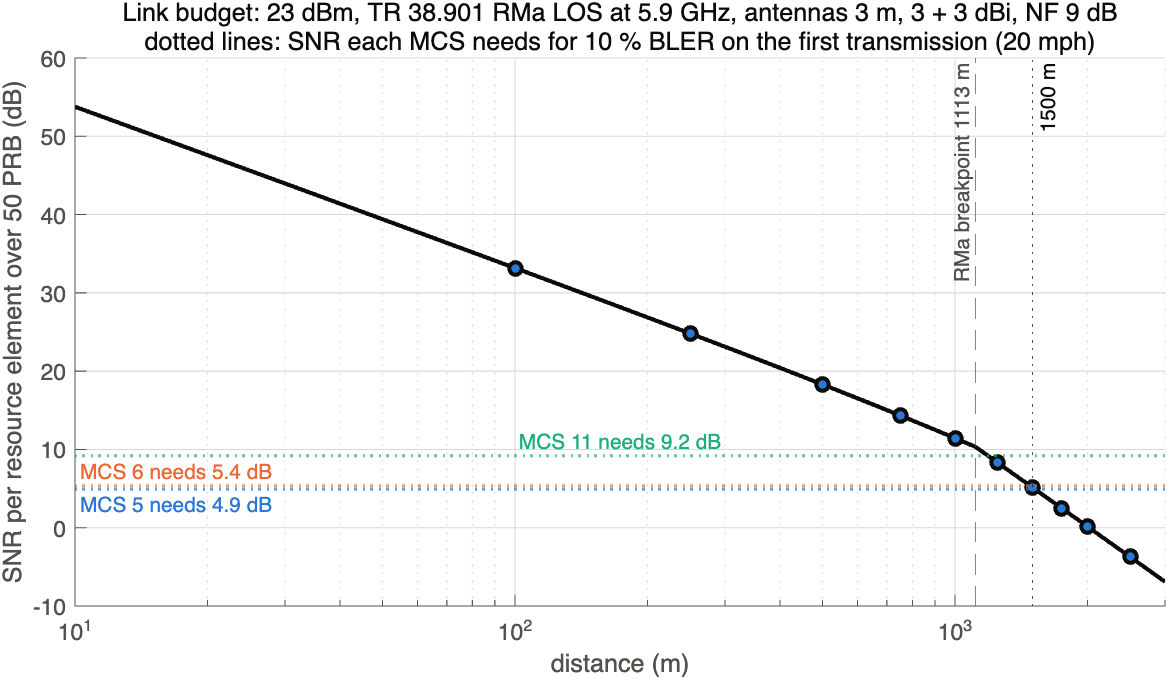
\includegraphics[width=0.9\textwidth]{figures/B1_snr_vs_distance.png}
  \caption{SNR against distance, with the SNR each MCS needs (10\% block
  error, first transmission, 20~mph) and the RMa breakpoint marked.}
  \label{fig:B1}
\end{figure}

\begin{table}[H]
\centering
\caption{Path loss, SNR and received power against distance.}
\label{tab:snr}
\small
\begin{tabular}{r r r r}
\toprule
\textbf{Distance} & \textbf{Path loss (RMa)} & \textbf{SNR per RE} & \textbf{Received power (50 PRB)} \\
\midrule
100~m  & 88.3~dB  & 33.2~dB  & $-59.3$~dBm \\
250~m  & 96.6~dB  & 24.8~dB  & $-67.6$~dBm \\
500~m  & 103.1~dB & 18.3~dB  & $-74.1$~dBm \\
750~m  & 107.1~dB & 14.3~dB  & $-78.1$~dBm \\
1000~m & 110.0~dB & 11.4~dB  & $-81.0$~dBm \\
1250~m & 113.1~dB & 8.3~dB   & $-84.1$~dBm \\
1500~m & 116.3~dB & 5.1~dB   & $-87.3$~dBm \\
1750~m & 119.0~dB & 2.5~dB   & $-90.0$~dBm \\
2000~m & 121.3~dB & 0.1~dB   & $-92.3$~dBm \\
2500~m & 125.2~dB & $-3.7$~dB & $-96.2$~dBm \\
\bottomrule
\end{tabular}
\end{table}

\subsection{How Speed Changes the PHY}
\label{sec:speed}

\begin{figure}[H]
  \centering
  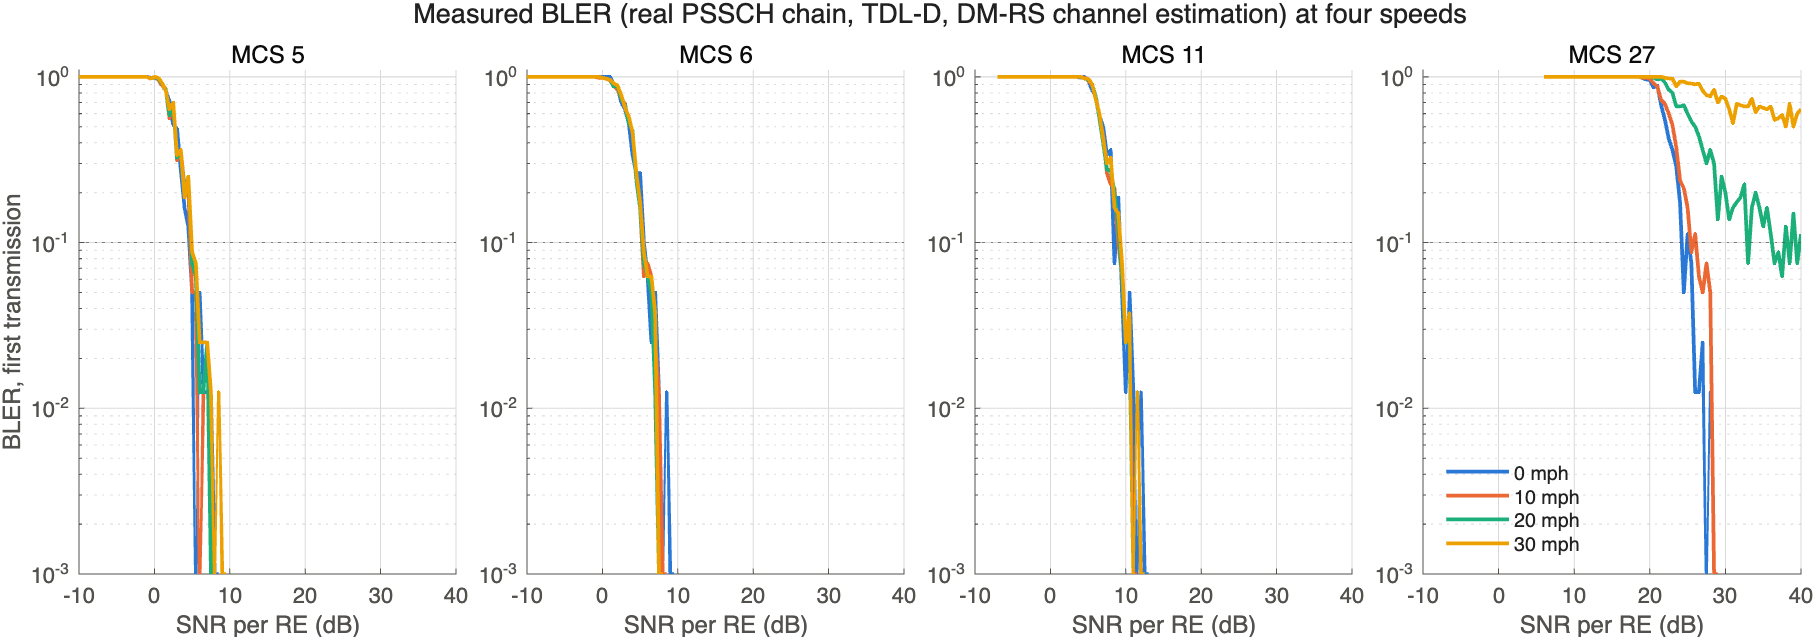
\includegraphics[width=\textwidth]{figures/B2_bler_by_speed.png}
  \caption{Measured block error rate at 0, 10, 20 and 30~mph.}
  \label{fig:B2}
\end{figure}

Speed here is the relative speed of the two vehicles, which sets the
Doppler spread. For MCS 5, 6 and 11 the curves barely move: QPSK and
16QAM at moderate code rates are robust to these Doppler levels, and the
line-of-sight path of TDL-D dominates. MCS~27 (64QAM, code rate 0.89) is
different. It needs high SNR at every speed, and from 20~mph its
first-transmission error rate never falls below 10\% at any SNR: the
channel changes between the two DM-RS symbols faster than linear
interpolation can follow.

\subsection{Range}
\label{sec:range}

\begin{figure}[H]
  \centering
  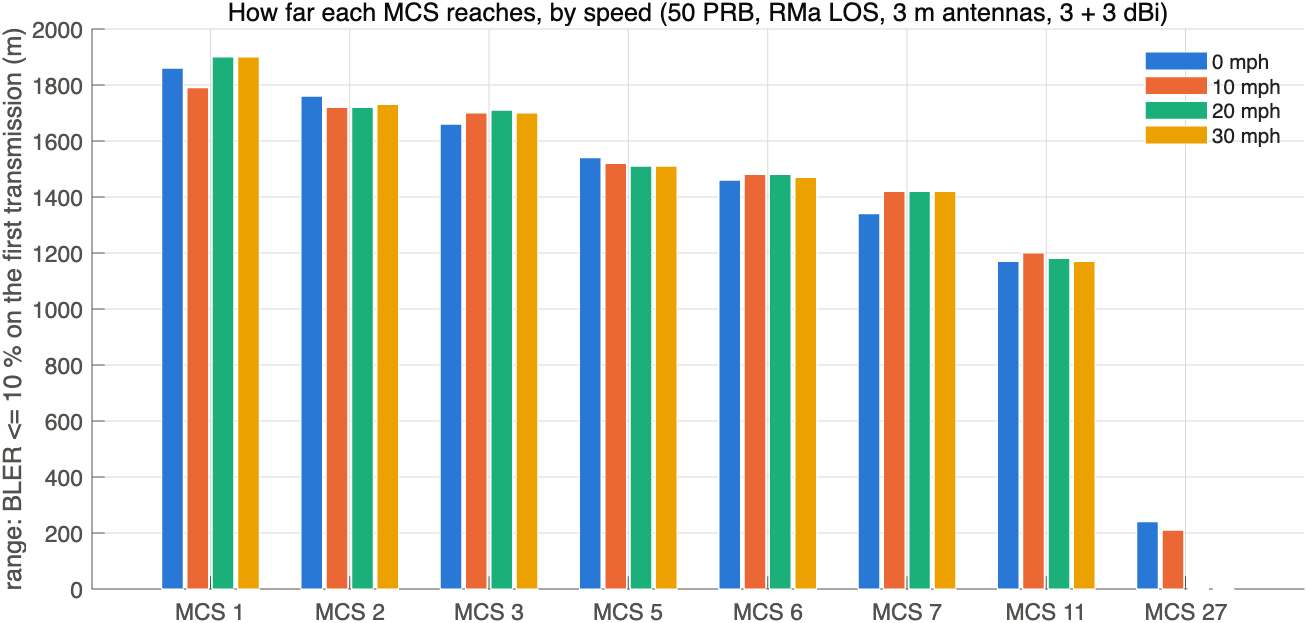
\includegraphics[width=0.9\textwidth]{figures/B3_range.png}
  \caption{How far each MCS reaches (first transmission decoded with at
  least 90\% probability).}
  \label{fig:B3}
\end{figure}

\begin{table}[H]
\centering
\caption{Range per MCS and speed.}
\label{tab:range}
\footnotesize\setlength{\tabcolsep}{3.5pt}
\begin{tabular}{c l c c c c c}
\toprule
\textbf{MCS} & \textbf{Modulation, rate} & \textbf{0 mph} & \textbf{10 mph} & \textbf{20 mph} & \textbf{30 mph} & \textbf{3 TX (20 mph)} \\
\midrule
1  & QPSK 0.15  & 1860~m & 1790~m & 1900~m & 1900~m & 2260~m \\
2  & QPSK 0.19  & 1760~m & 1720~m & 1720~m & 1730~m & 2160~m \\
3  & QPSK 0.25  & 1660~m & 1700~m & 1710~m & 1700~m & 2100~m \\
\textbf{5}  & QPSK 0.37  & \textbf{1540~m} & \textbf{1520~m} & \textbf{1510~m} & \textbf{1510~m} & 1930~m \\
\textbf{6}  & QPSK 0.44  & \textbf{1460~m} & \textbf{1480~m} & \textbf{1480~m} & \textbf{1470~m} & 1900~m \\
7  & QPSK 0.51  & 1340~m & 1420~m & 1420~m & 1420~m & 1840~m \\
\textbf{11} & 16QAM 0.37 & \textbf{1170~m} & \textbf{1200~m} & \textbf{1180~m} & \textbf{1170~m} & 1620~m \\
\textbf{27} & 64QAM 0.89 & \textbf{240~m}  & \textbf{210~m}  & --- & --- & 910~m \\
\bottomrule
\end{tabular}
\end{table}

\begin{itemize}[nosep]
  \item \textbf{MCS~5 survives at 1500~m} at every speed on its first
  transmission.
  \item \textbf{The lower MCS reach further}, but by less than in free
  space: MCS 1--3 reach 1.7--1.9~km on one transmission and 2.1--2.3~km
  with retransmissions. Beyond the RMa breakpoint every extra dB of
  margin buys less distance, because the loss grows at 40~dB per decade.
  \item \textbf{MCS~27 works only at short range}, and from 20~mph only
  with retransmissions.
\end{itemize}

\subsection{Throughput against Distance}
\label{sec:linkthr}

\begin{figure}[H]
  \centering
  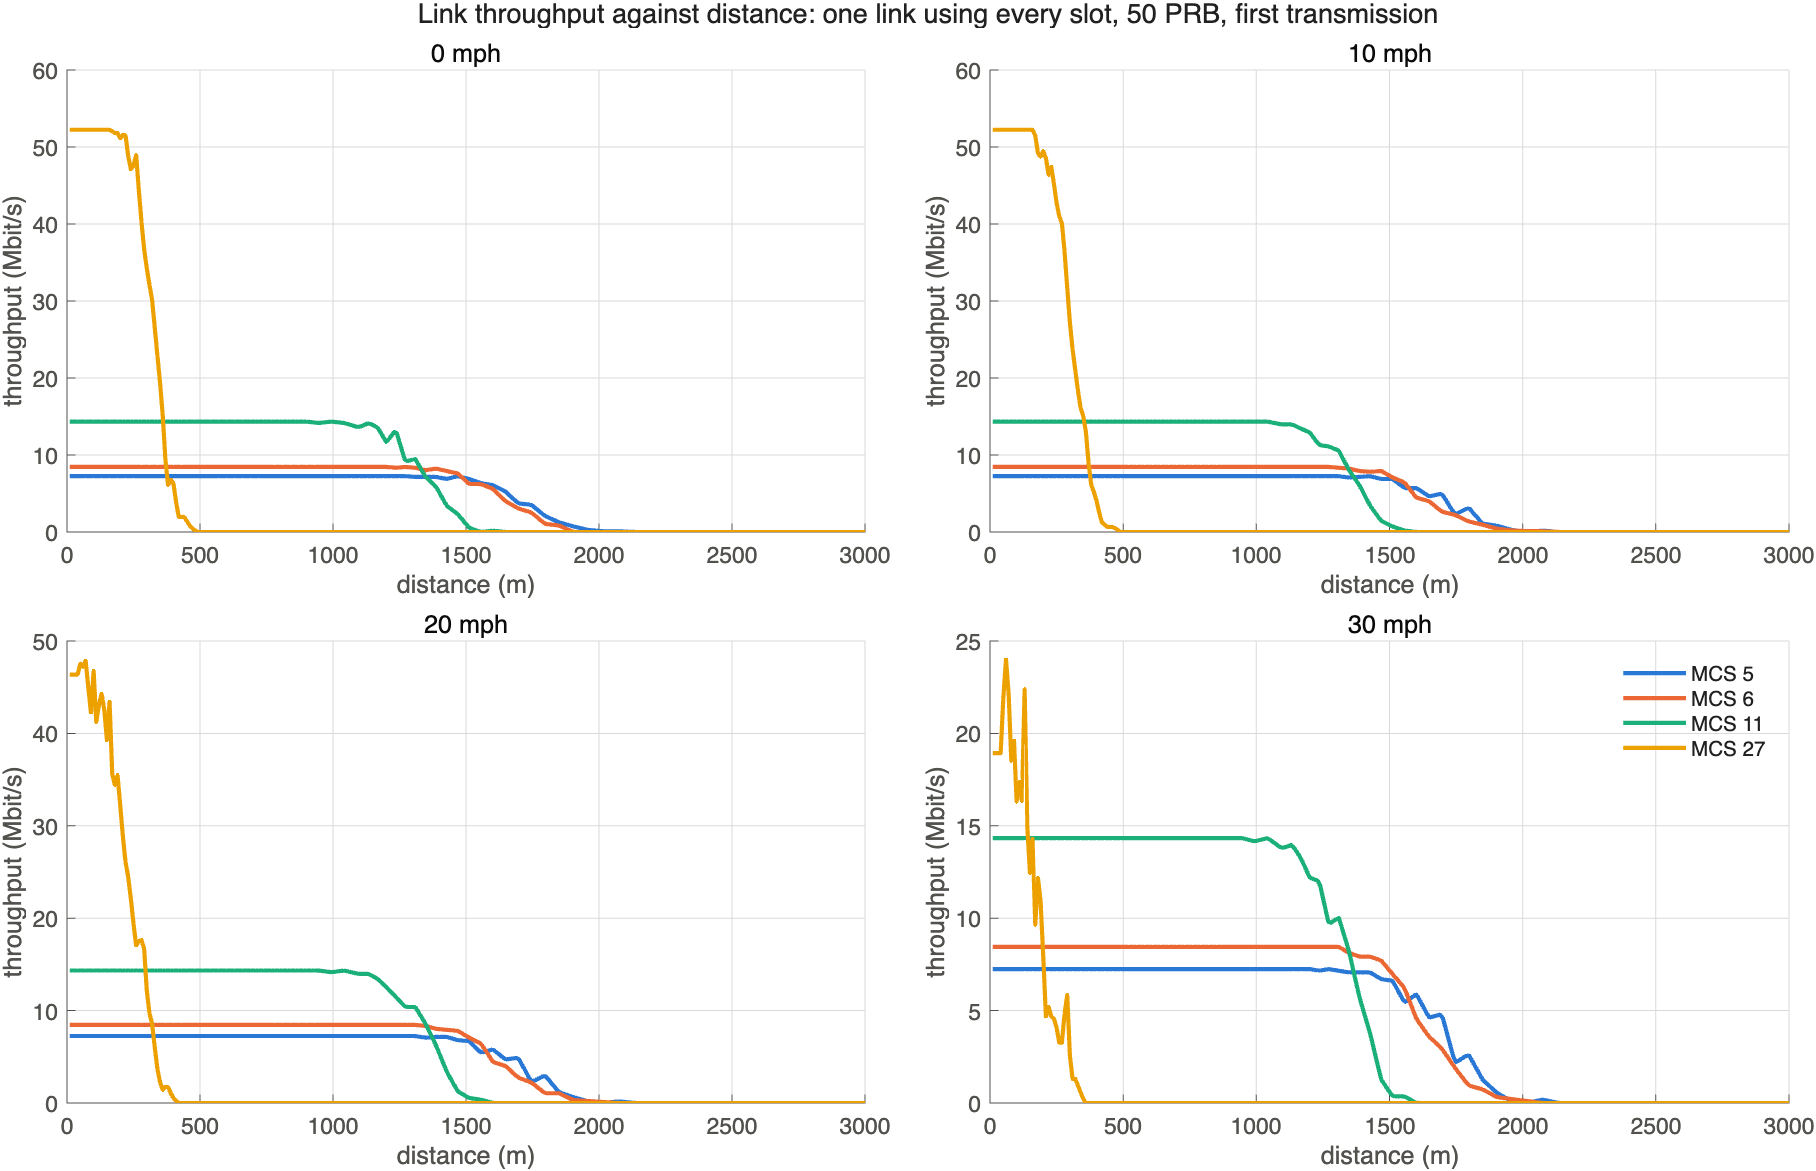
\includegraphics[width=\textwidth]{figures/B4_throughput.png}
  \caption{Link throughput against distance at each speed: one link
  using every slot over the whole 50-PRB channel, first transmission
  only.}
  \label{fig:B4}
\end{figure}

The throughput in Fig.~\ref{fig:B4} is transport-block size $\times$
$(1 - \mathrm{BLER})$ / 0.5~ms. Each curve is flat at its peak while the
link is clean, then falls over a few hundred metres as the SNR runs out.

\begin{table}[H]
\centering
\caption{Link throughput per MCS.}
\label{tab:linkthr}
\small
\begin{tabularx}{\textwidth}{c X c c}
\toprule
\textbf{MCS} & \textbf{Peak (error-free)} & \textbf{Held (within 5\% of peak) to} & \textbf{Falls to zero by} \\
\midrule
5  & 7.2~Mbit/s  & $\sim$1450~m & $\sim$2100~m \\
6  & 8.4~Mbit/s  & $\sim$1380~m & $\sim$2000~m \\
11 & 14.3~Mbit/s & $\sim$1150~m & $\sim$1580~m \\
27 & 52.2~Mbit/s (0--10 mph); $\sim$48~Mbit/s at 20~mph; $\sim$24~Mbit/s at 30~mph & 60--220~m & $\sim$400~m \\
\bottomrule
\end{tabularx}
\end{table}

\textbf{Choosing an MCS} is therefore a choice of distance:
\begin{itemize}[nosep]
  \item MCS~27 for 25--50~Mbit/s inside about 200~m;
  \item MCS~11 for 14~Mbit/s to about 1.15~km;
  \item MCS 5--6 for 7--8~Mbit/s to about 1.4--1.5~km.
\end{itemize}
These are rates for \textbf{one link holding the whole channel in every
slot}. What a UE gets when many share the channel under sensing is in
Section~\ref{sec:bcthr}.

\subsection{Latency and Reliability against Distance, per PQI}
\label{sec:linklat}

At link level there are no other users, so latency is the Mode-2 window
plus whatever retransmission the radio needs, plus the 3-slot pipeline:
\begin{itemize}[nosep]
  \item the first transmission is drawn uniformly in $[n + 5, n +
  \mathrm{PDB} - 3]$ slots;
  \item one blind retransmission follows within 31 slots (and before
  $\Ttwo$), and is soft-combined with the first;
  \item the rows of Figs.~\ref{fig:B5} and~\ref{fig:B6} are the PDBs of
  the broadcast PQIs 55, 56, 57 and 58 (10, 20, 25 and 100~ms).
\end{itemize}

\begin{figure}[H]
  \centering
  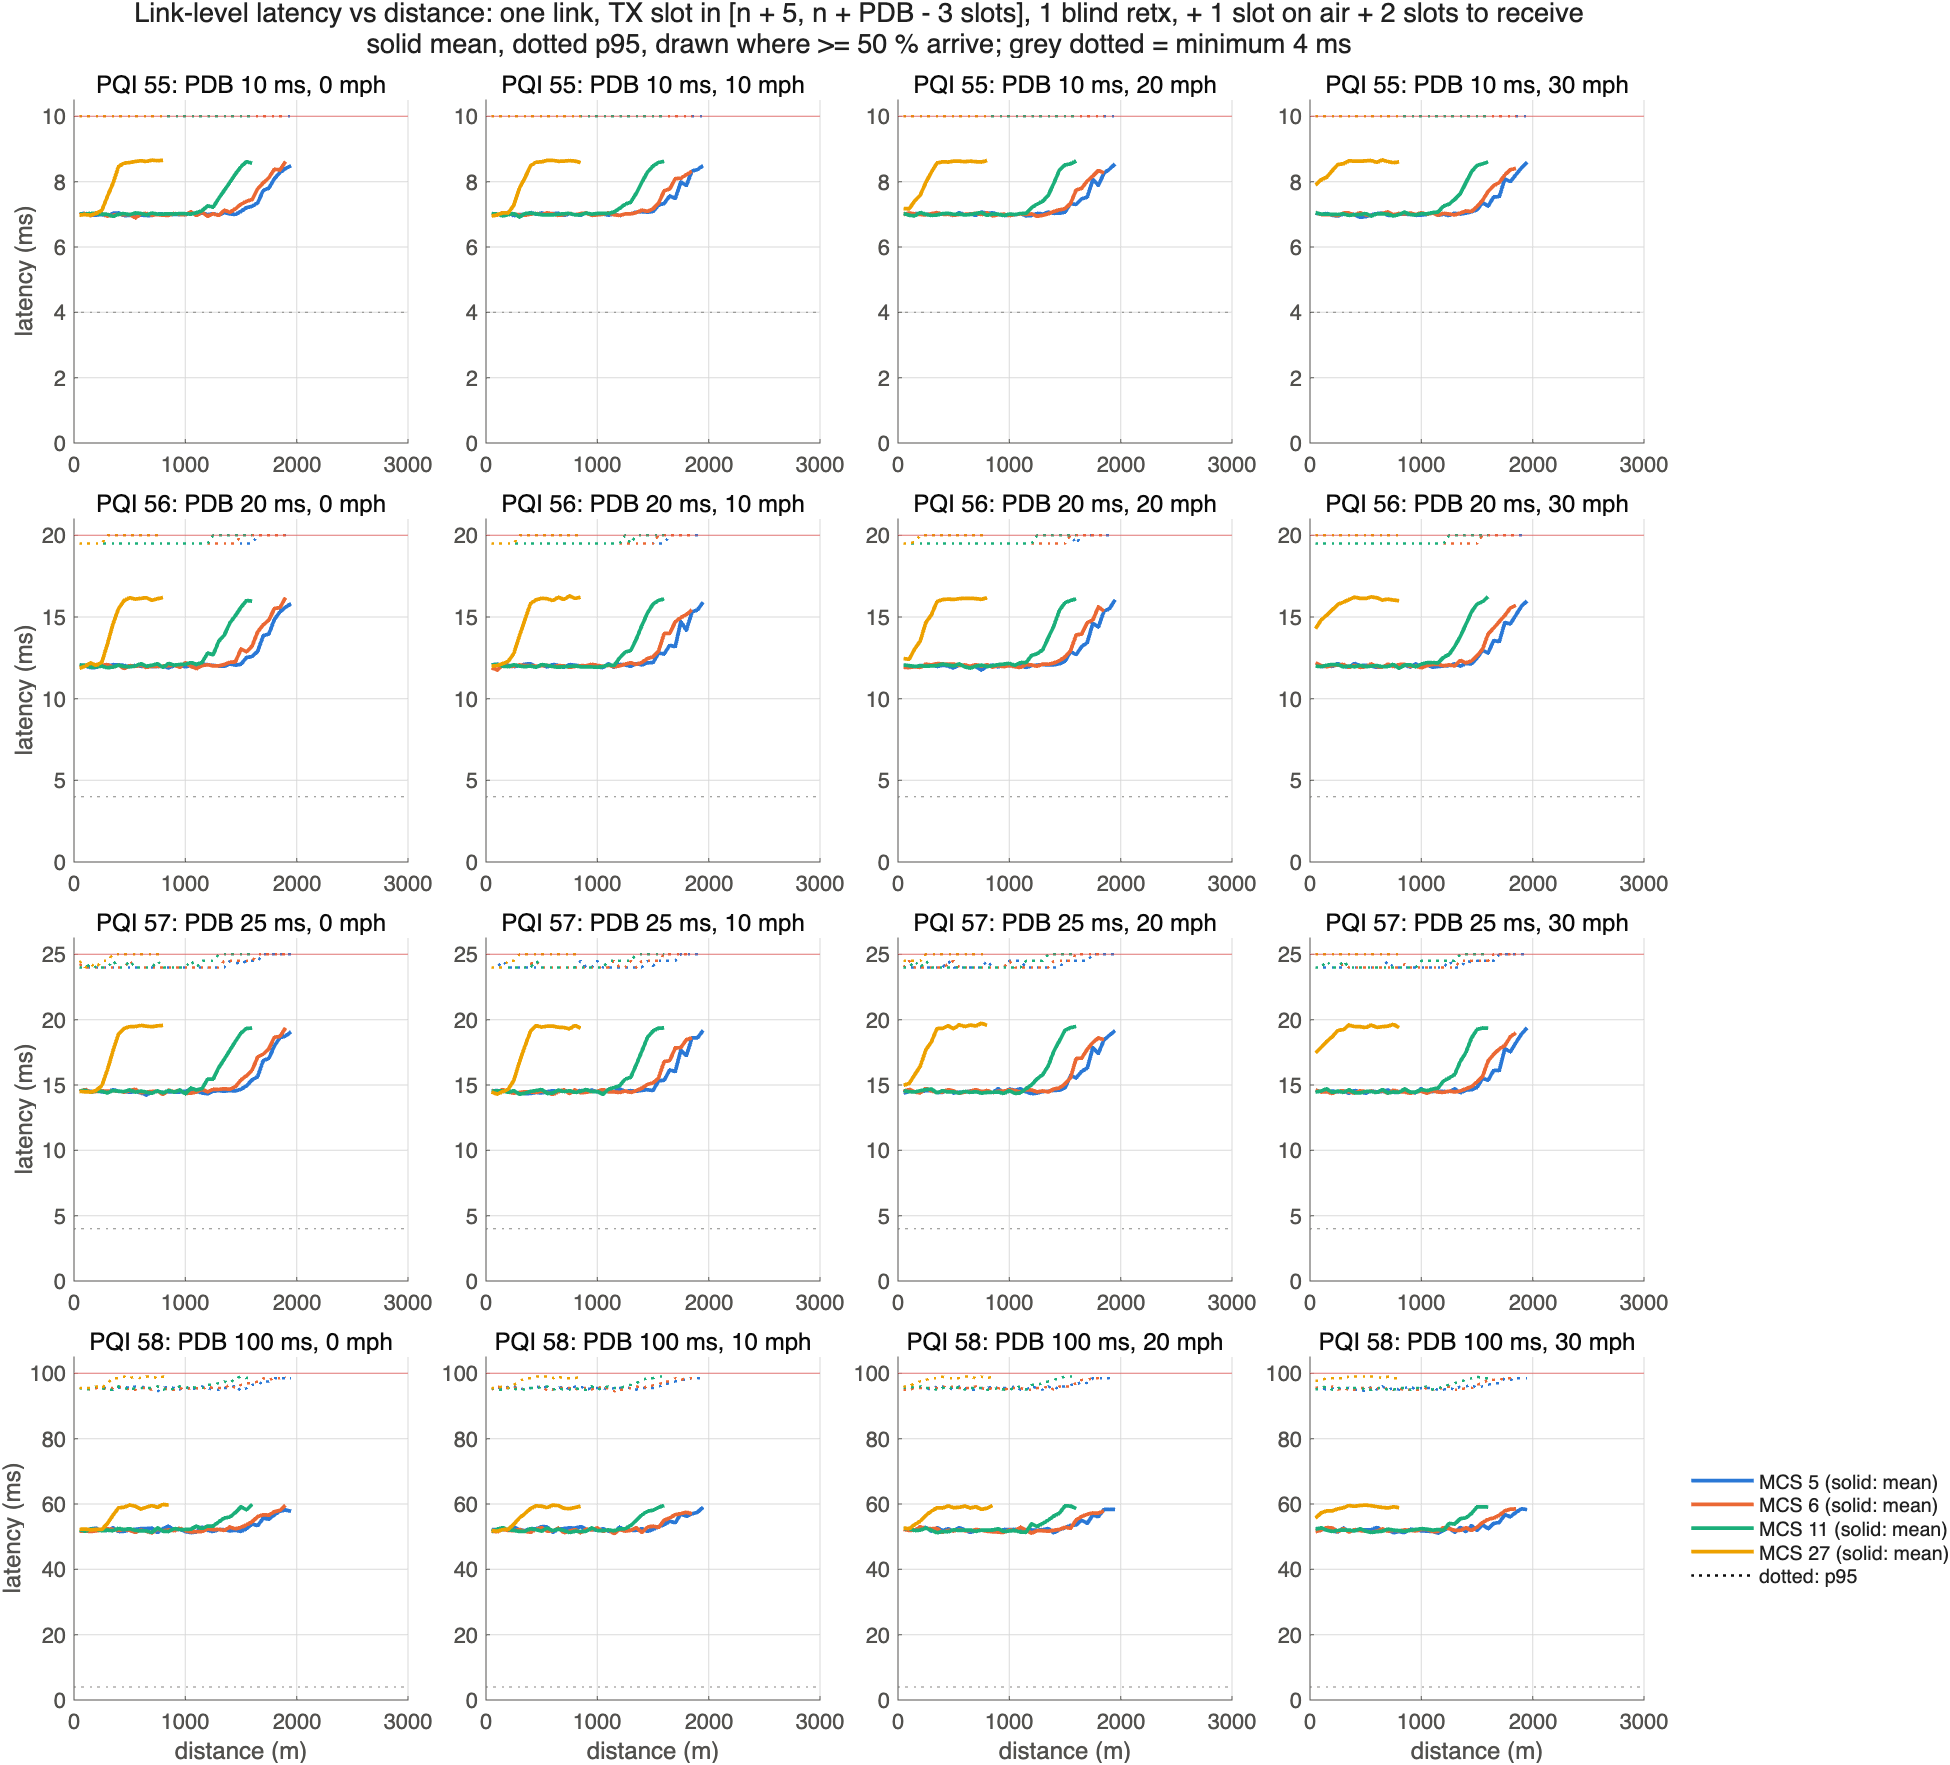
\includegraphics[width=\textwidth]{figures/B5_latency.png}
  \caption{Latency against distance, one row per PQI, one column per
  speed. Solid: mean; dotted: 95th percentile, drawn where at least half
  the packets arrive. Red: the PDB; grey dotted: the 4~ms floor.}
  \label{fig:B5}
\end{figure}

\begin{table}[H]
\centering
\caption{Link-level latency per PQI.}
\label{tab:linklat}
\small
\begin{tabular}{l c c c}
\toprule
\textbf{PQI (PDB)} & \textbf{Mean inside the range} & \textbf{95th percentile} & \textbf{Mean near the range edge} \\
\midrule
55 (10~ms)  & 7.0~ms  & 10~ms        & $\sim$8.5~ms \\
56 (20~ms)  & 12.0~ms & 19.5~ms      & $\sim$16~ms \\
57 (25~ms)  & 14.5~ms & 24--24.5~ms  & $\sim$19.5~ms \\
58 (100~ms) & 52~ms   & 95--96~ms    & $\sim$59~ms \\
\bottomrule
\end{tabular}
\end{table}

\begin{itemize}[nosep]
  \item \textbf{Inside the range the mean is the middle of the window
  plus 1.5~ms}, for every MCS and every speed, exactly the Part~A
  prediction.
  \item \textbf{Towards the range edge the mean rises}, because more
  packets need the retransmission, which comes later.
  \item \textbf{MCS~27's mean is higher everywhere it works}, because at
  64QAM it usually needs its retransmission.
\end{itemize}

\begin{figure}[H]
  \centering
  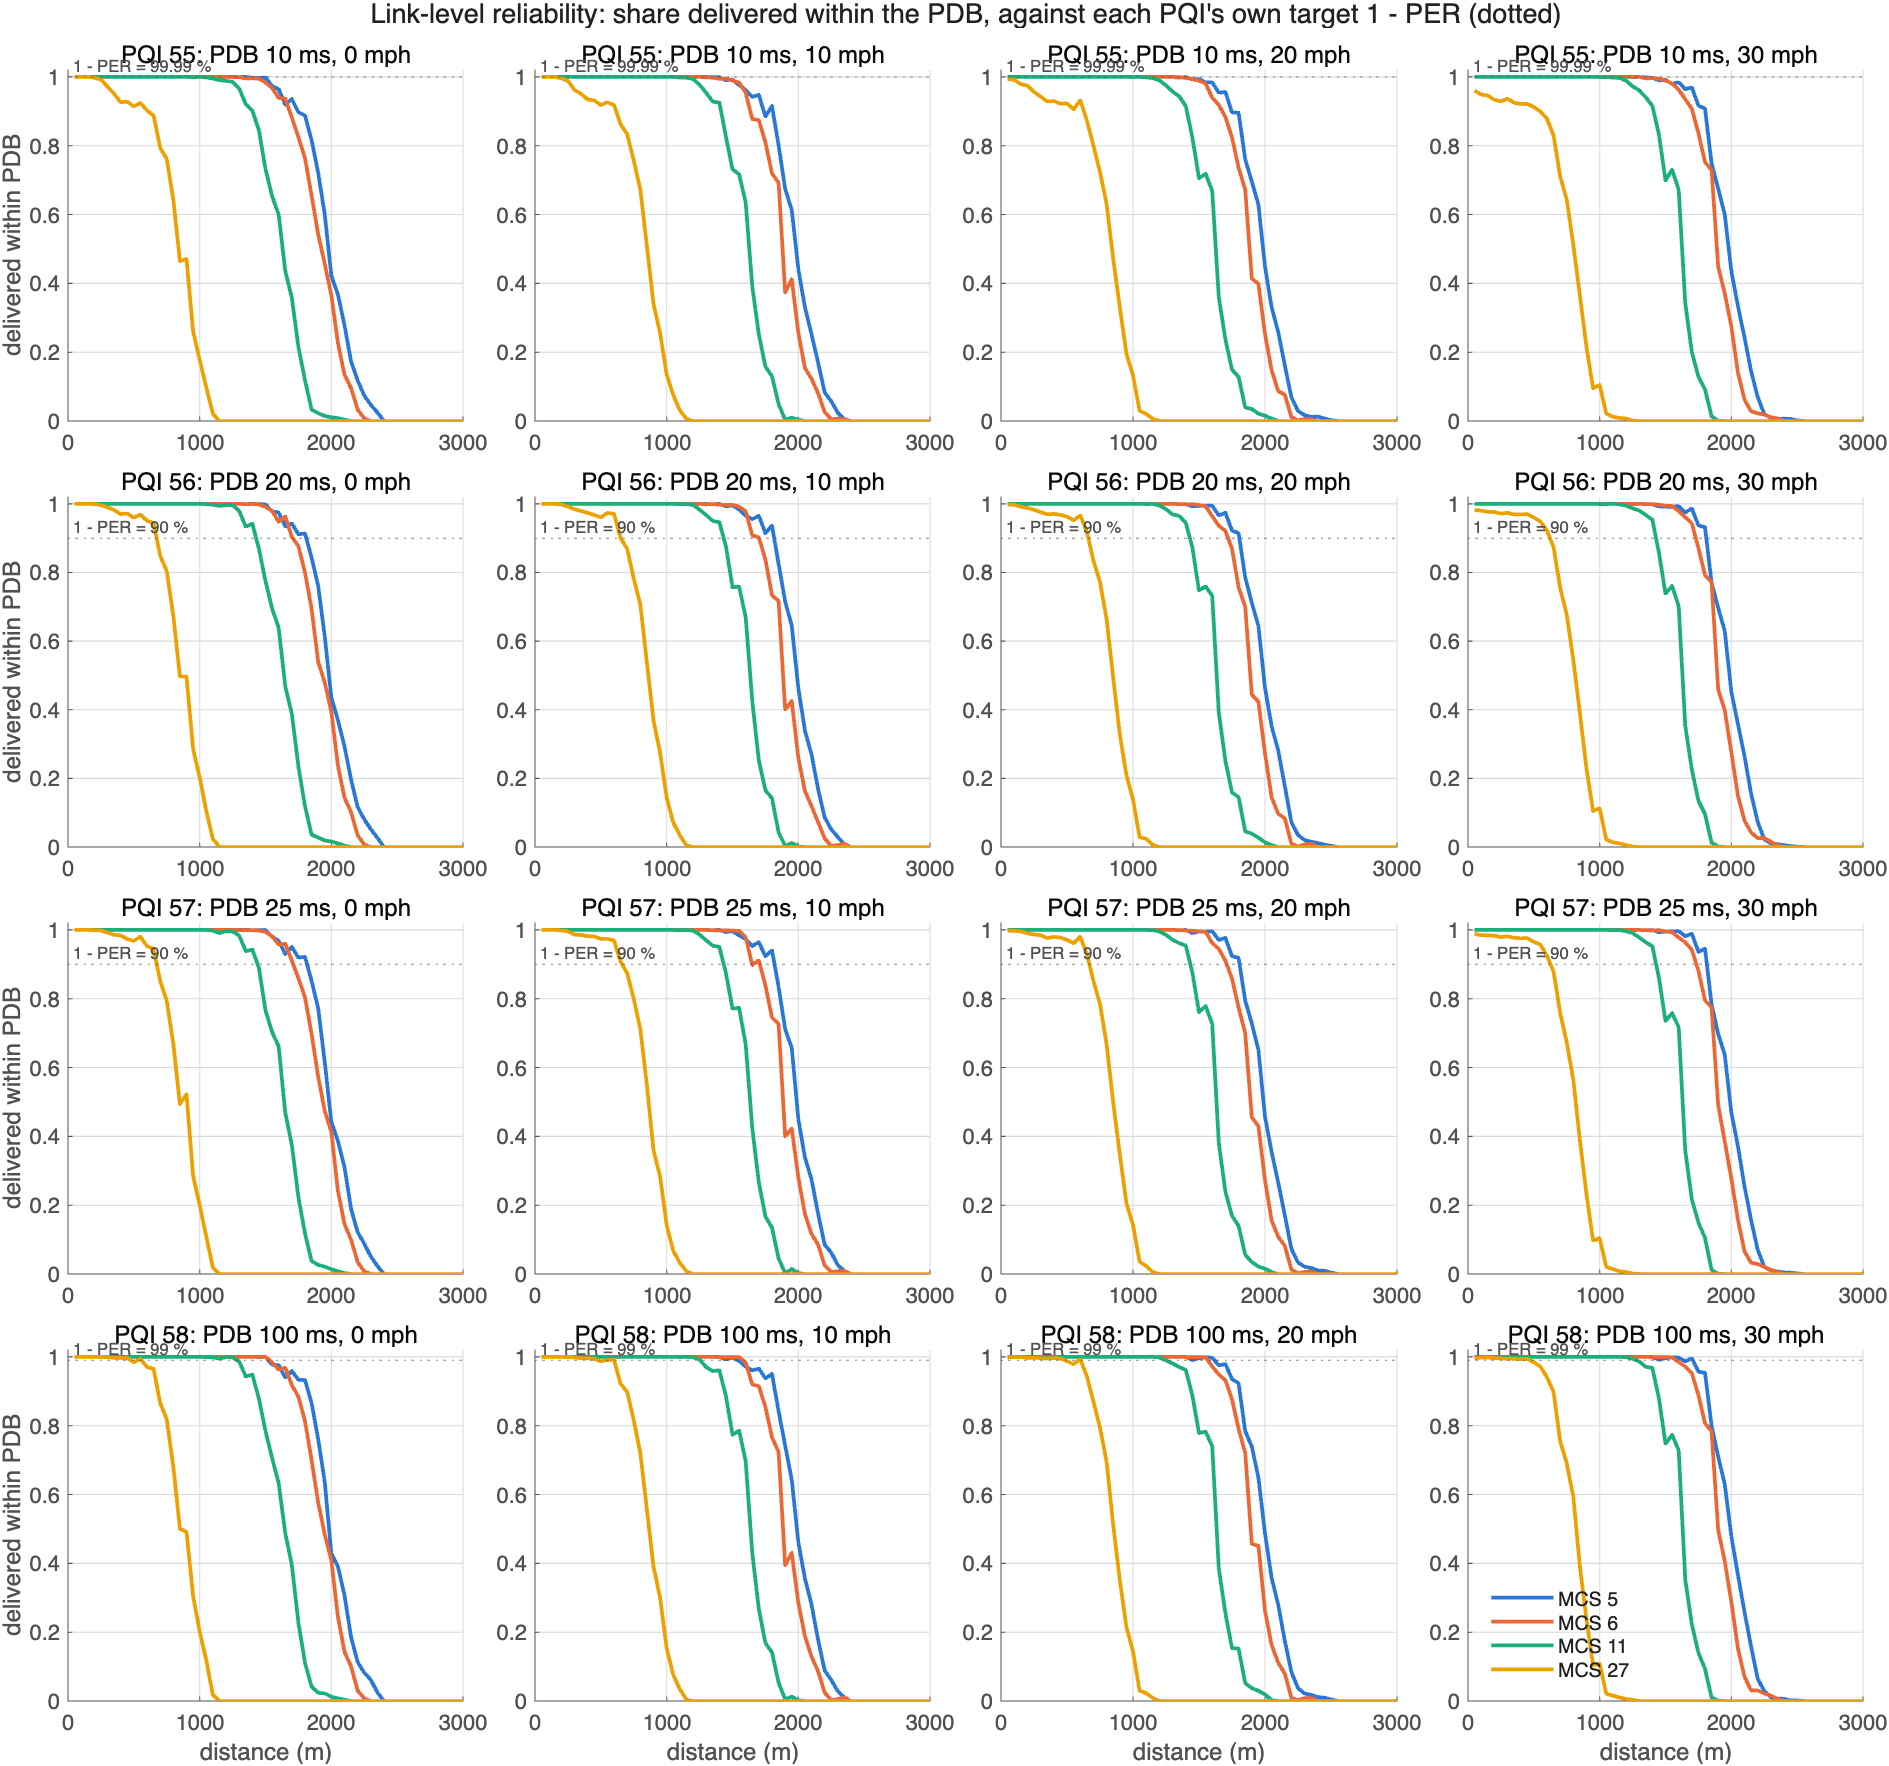
\includegraphics[width=\textwidth]{figures/B6_prr.png}
  \caption{Share of packets delivered within the PDB against distance,
  with each PQI's own target $1 - \mathrm{PER}$ dotted.}
  \label{fig:B6}
\end{figure}

\begin{table}[H]
\centering
\caption{Distance up to which each MCS meets the PQI's target at 20~mph.}
\label{tab:linkrel}
\footnotesize\setlength{\tabcolsep}{3.5pt}
\begin{tabular}{c c c c c}
\toprule
\textbf{MCS} & \textbf{PQI 55} (99.99\%, 10 ms) & \textbf{PQI 56} (90\%, 20 ms) & \textbf{PQI 57} (90\%, 25 ms) & \textbf{PQI 58} (99\%, 100 ms) \\
\midrule
5  & 1300~m$^{*}$ & 1800~m & 1800~m & 1600~m \\
6  & 1300~m$^{*}$ & 1700~m & 1700~m & 1550~m \\
11 & 950~m$^{*}$  & 1400~m & 1400~m & 1250~m \\
27 & ---          & 650~m  & 650~m  & 450~m \\
\bottomrule
\multicolumn{5}{l}{\footnotesize $^{*}$ 4000 packets per point: 99.99\% means ``no failure seen in 4000'', not a demonstrated $10^{-4}$.}
\end{tabular}
\end{table}

With one blind retransmission, every MCS reaches further at the 90\% and
99\% targets than its single-transmission range in
Table~\ref{tab:range}.

\subsection{Speed at a Glance}

\begin{figure}[H]
  \centering
  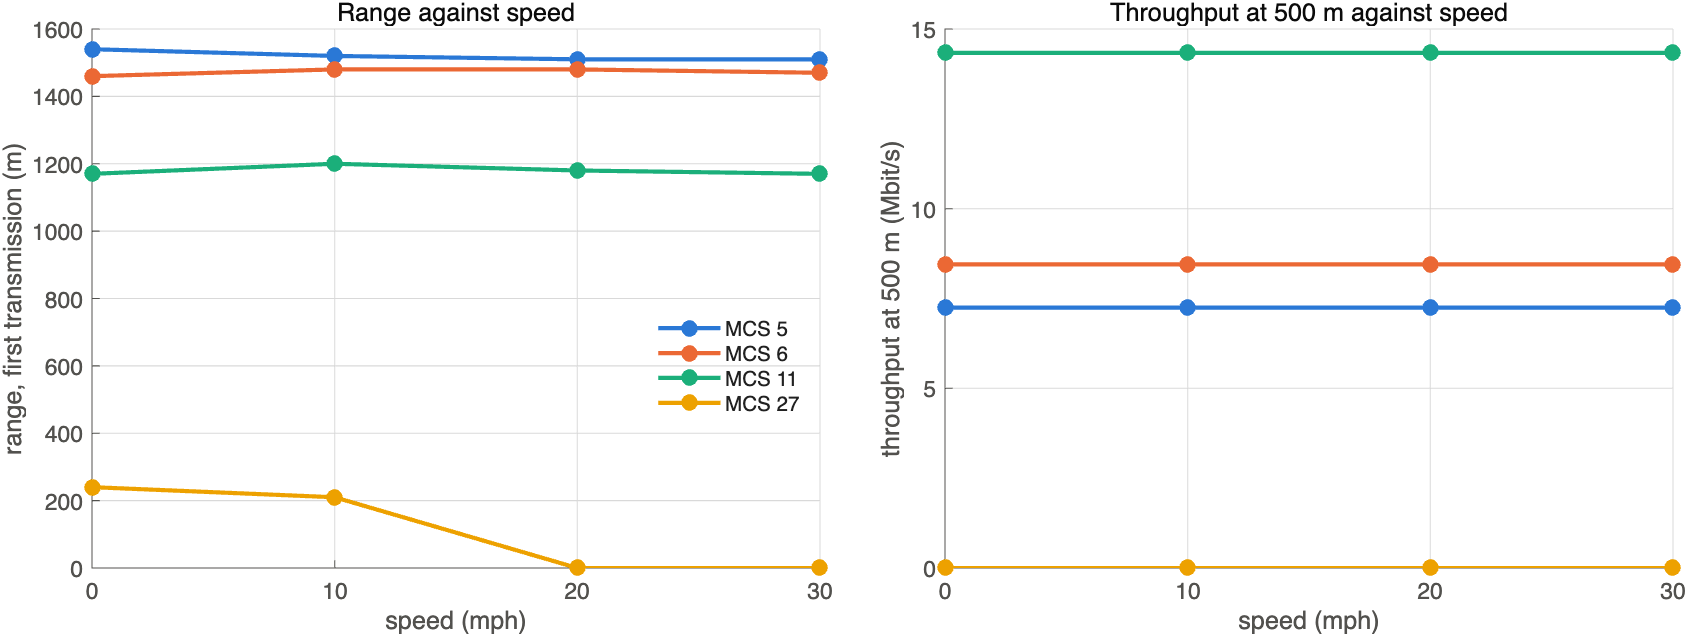
\includegraphics[width=\textwidth]{figures/B7_speed_effect.png}
  \caption{Range and throughput at 500~m against speed.}
  \label{fig:B7}
\end{figure}

Between 0 and 30~mph, speed changes the range of MCS 5, 6 and 11 by
under 5\% (Fig.~\ref{fig:B7}). Only MCS~27 is sensitive: its
single-transmission throughput at short range halves by 30~mph.

\subsection{Part B Summary}

With RMa line-of-sight propagation, antennas at 3~m on the machinery,
3~dBi each and a 9~dB noise figure (TR~37.885 \cite{ref:37885}), MCS~5
reaches 1500~m on its first transmission, and MCS 1--3 reach 1.7--1.9~km.
\begin{itemize}[nosep]
  \item \textbf{Throughput:} 7--8~Mbit/s to about 1.4--1.5~km (MCS 5--6),
  14~Mbit/s to about 1.15~km (MCS~11), and 25--50~Mbit/s only inside
  about 200~m (MCS~27).
  \item \textbf{Speed:} up to 30~mph it barely matters, except for MCS~27.
  \item \textbf{Reliability with one blind retransmission:} the 90\% PQIs
  (56, 57) are met to 1.8~km at MCS~5, the 99\% PQI~58 to 1.6~km, and
  PQI~55's 99.99\% to about 1.3~km.
  \item \textbf{Latency} is the middle of the Mode-2 window plus 1.5~ms
  wherever the link is good.
\end{itemize}

%==========================================================================
\newpage
\section{Part C: Many UEs in a 1~km $\times$ 1~km Field}
\label{sec:partC}

Parts A and B looked at one UE choosing resources and one link carrying
them. Part~C puts many UEs in one field, all sensing, reserving and
transmitting at once. Now the losses come from each other, not from
distance.

\subsection{The Traffic, Stated before Deployment}
\label{sec:traffic}

Every UE runs all five broadcast PQIs at once, each as the service
Table~5.4.4-1 names for it \cite{ref:23287}. Each flow passes when at
least $1 - \mathrm{PER}$ of its packets arrive within its PDB at every
intended receiver; the target is set by the PQI, not by a generic 90\%.
The total offered load is \textbf{48~kbit/s per UE}.

\begin{table}[H]
\centering
\caption{Traffic carried by every UE.}
\label{tab:flows}
\footnotesize\setlength{\tabcolsep}{3.5pt}
\begin{tabularx}{\textwidth}{X c l c c c c c c}
\toprule
\textbf{Flow} & \textbf{PQI} & \textbf{Arrival} & \textbf{Size} & \textbf{Offered} & \textbf{PDB} & \textbf{PER} & \textbf{Target} & \textbf{Prio.} \\
\midrule
Sensor information sharing & 58 & every 100~ms & 300~B & 24~kbit/s & 100~ms & $10^{-2}$ & 99\% & 4 \\
Platooning informative exchange & 56 & every 100~ms & 200~B & 16~kbit/s & 20~ms & $10^{-1}$ & 90\% & 6 \\
Platooning, report to RSU & 59 & every 500~ms & 200~B & 3.2~kbit/s & 500~ms & $10^{-1}$ & 90\% & 6 \\
Cooperative lane change & 55 & Poisson, 500~ms & 200~B & 3.2~kbit/s & 10~ms & $10^{-4}$ & 99.99\% & 3 \\
Lane change, lower automation & 57 & Poisson, 1~s & 200~B & 1.6~kbit/s & 25~ms & $10^{-1}$ & 90\% & 5 \\
\bottomrule
\end{tabularx}
\end{table}

\begin{table}[H]
\centering
\caption{System-level simulation settings.}
\label{tab:sls}
\small
\begin{tabularx}{\textwidth}{l X}
\toprule
\textbf{Setting} & \textbf{Value} \\
\midrule
Field & 1~km $\times$ 1~km \\
Densities & 5, 10, 15, 20, 30, 40, 50, 75 and 100~UE/km$^2$ \\
Drops & 3 independent drops per density (seeds 7, 11, 23) \\
Cast type & broadcast; intended receivers are all UEs within 500~m of the sender \\
MCS & 11 (16QAM); Part~B gives it about 1180~m of range, so every intended receiver is within reach of the radio \\
Resource selection & sensing-based SPS (Part~A), $\Prsvp = 100$~ms, one blind retransmission, $\Tone = 5$ slots, $\Ttwo = \mathrm{PDB} - 3$ slots \\
Latency & transmission slot $-$ arrival $+$ 3 slots (Eq.~\eqref{eq:latency}) \\
Radio & the Part~B link (RMa LOS, 3~m antennas, 3 + 3~dBi, NF 9~dB) and the TDL-D block-error tables measured at 20~mph; interference from every overlapping transmission is added to the noise \\
Length & 5~s (10\,000 slots) per run \\
\bottomrule
\end{tabularx}
\end{table}

\paragraph{How the UEs are distributed.} UE positions are a
\textbf{homogeneous Poisson point process (PPP)}:
\begin{itemize}[nosep]
  \item the number of UEs in the 1~km$^2$ field is $N \sim
  \mathrm{Poisson}(\lambda)$, with $\lambda$ the density per km$^2$;
  \item given $N$, each UE is placed independently and uniformly over the
  field;
  \item each seed is a new, independent drop.
\end{itemize}

\begin{table}[H]
\centering
\caption{UE count of every drop, and mean neighbours within 500~m.}
\label{tab:drops}
\small
\begin{tabular}{r c c}
\toprule
\textbf{Density (UE/km$^2$)} & \textbf{$N$ in the three drops} & \textbf{Mean neighbours within 500~m} \\
\midrule
5   & 5, 6, 8       & 2.2 \\
10  & 10, 11, 14    & 4.9 \\
15  & 15, 16, 20    & 7.6 \\
20  & 20, 22, 26    & 9.3 \\
30  & 30, 32, 38    & 14.7 \\
40  & 41, 42, 49    & 20.7 \\
50  & 51, 53, 60    & 26.0 \\
75  & 76, 78, 87    & 38.7 \\
100 & 101, 104, 114 & 51.0 \\
\bottomrule
\end{tabular}
\end{table}

A UE far from the edges would have $\lambda \pi r^2$ neighbours within
$r = 500$~m (23.6 at 30~UE/km$^2$). In a 1~km field most UEs are near an
edge and have fewer: about 62\% of that.

\begin{figure}[H]
  \centering
  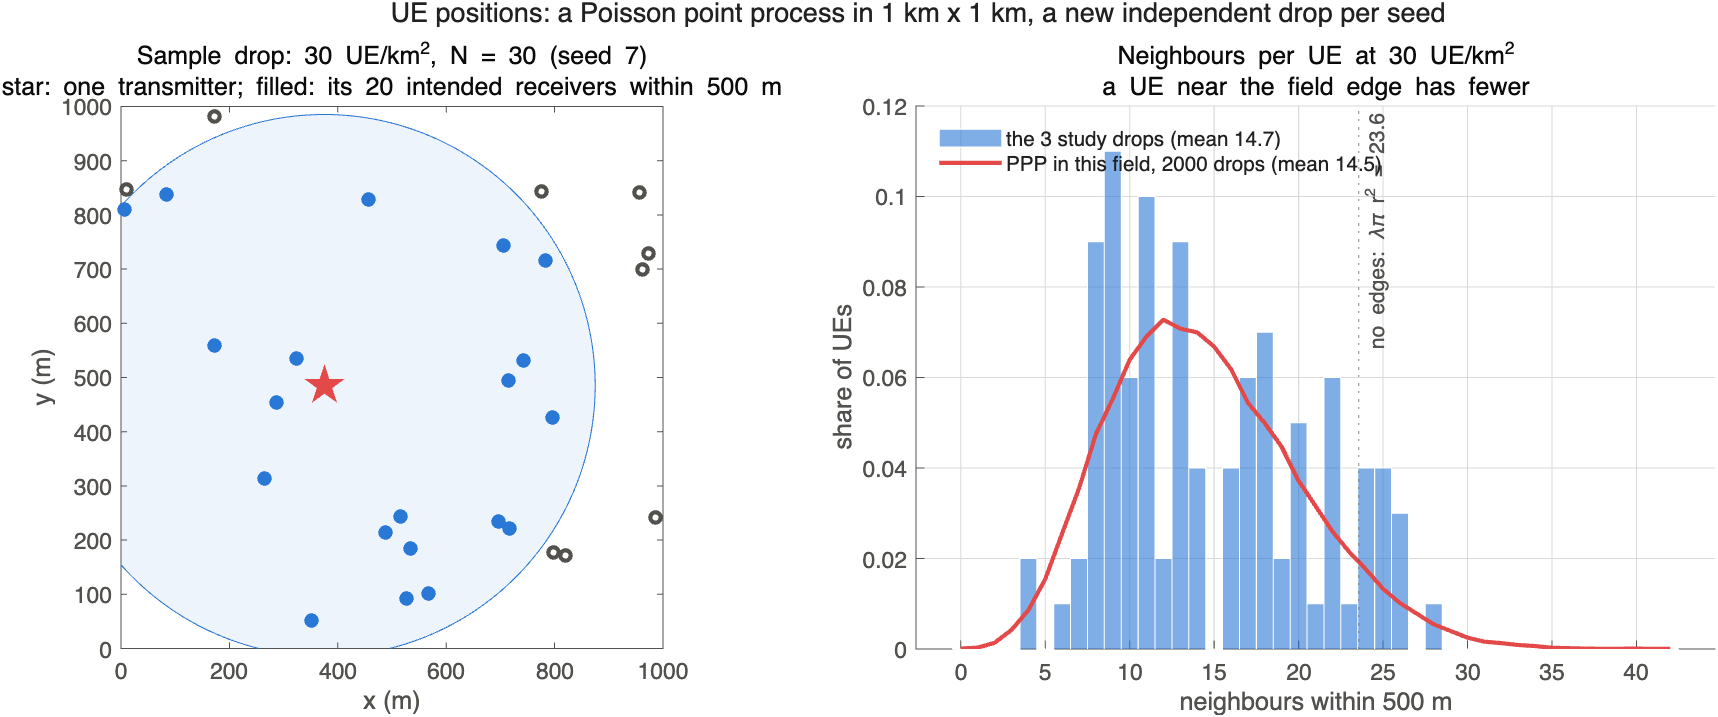
\includegraphics[width=\textwidth]{figures/C1_deployment.png}
  \caption{One sample drop, and how many neighbours a UE has. Left: the
  30~UE/km$^2$ drop of seed 7 (star: one transmitter; filled: its 20
  intended receivers within 500~m). Right: neighbour count across the
  three study drops at 30~UE/km$^2$ (bars) against 2000 simulated PPP
  drops of the same field (red); the dotted line is the edge-free value
  $\lambda\pi r^2$.}
  \label{fig:C1}
\end{figure}

\paragraph{How a UE carries five flows, and what it costs.} The simulator
gives each UE one grant, and its MAC multiplexes all five flows into it
in priority order. Two consequences shape everything below:
\begin{itemize}[nosep]
  \item \textbf{Every transmission fills the whole channel.} The grant is
  sized for one reservation period of all five flows (about 1100~B). The
  widest transport block at MCS~11 holds 896~B, so all 5 sub-channels are
  taken: measured, 361 of 361 transmissions in a sample run. Two UEs
  therefore never share a slot side by side in frequency; any two
  transmissions in the same slot collide.
  \item \textbf{The grant is reselected often.} The 10, 20 and 25~ms
  flows (PQIs 55, 56, 57) often cannot wait for the next reserved slot of
  a 100~ms grant, and each such packet forces a reselection: about 6.5
  per UE per second. A grant therefore lives about 150~ms, not the
  1.6~s of Part~A's single-flow SPS, and sensing has less advance notice
  to work with.
\end{itemize}
A real UE could hold several grants, one per flow class. That is outside
this simulator, and it is the first thing to change for a deployment
carrying 10~ms traffic.

\subsection{Reliability, Each Flow against its Own Target}
\label{sec:rel}

\begin{figure}[H]
  \centering
  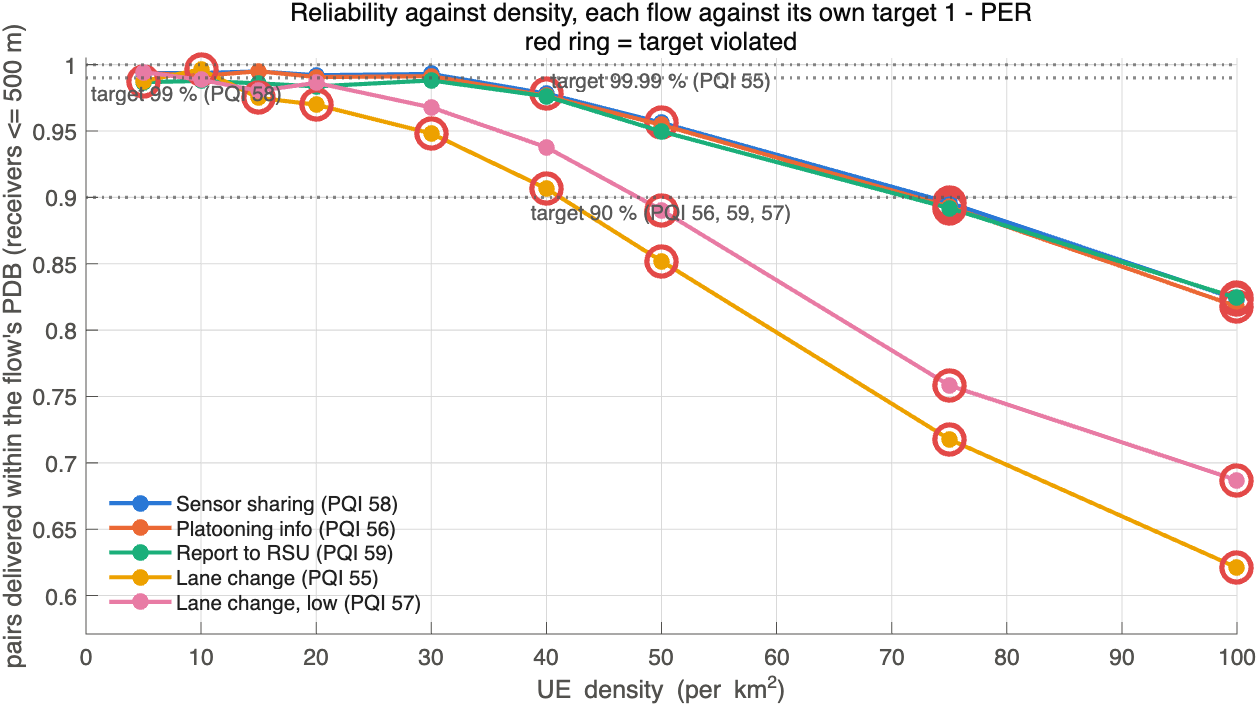
\includegraphics[width=\textwidth]{figures/C2_reliability.png}
  \caption{Share of (packet, receiver) pairs delivered within the PDB
  against density. Dotted: the three targets; red ring: target violated.}
  \label{fig:C2}
\end{figure}

\begin{table}[H]
\centering
\caption{Delivered within the PDB, per flow and density.}
\label{tab:rel}
\footnotesize\setlength{\tabcolsep}{3.5pt}
\begin{tabular}{r c c c c c}
\toprule
\textbf{Density} & \textbf{PQI 58 (99\%)} & \textbf{PQI 56 (90\%)} & \textbf{PQI 59 (90\%)} & \textbf{PQI 55 (99.99\%)} & \textbf{PQI 57 (90\%)} \\
\midrule
5   & 99.37\% \pass & 99.38\% \pass & 98.68\% \pass & 98.76\% \fail & 99.44\% \pass \\
10  & 99.37\% \pass & 99.15\% \pass & 98.77\% \pass & 99.65\% \fail & 98.85\% \pass \\
15  & 99.49\% \pass & 99.50\% \pass & 98.59\% \pass & 97.50\% \fail & 98.02\% \pass \\
20  & 99.20\% \pass & 99.06\% \pass & 98.36\% \pass & 96.98\% \fail & 98.63\% \pass \\
30  & 99.30\% \pass & 99.13\% \pass & 98.81\% \pass & 94.82\% \fail & 96.78\% \pass \\
40  & 97.82\% \fail & 97.64\% \pass & 97.61\% \pass & 90.66\% \fail & 93.78\% \pass \\
50  & 95.62\% \fail & 95.46\% \pass & 94.97\% \pass & 85.19\% \fail & 89.04\% \fail \\
75  & 89.60\% \fail & 89.30\% \fail & 89.19\% \fail & 71.78\% \fail & 75.84\% \fail \\
100 & 82.33\% \fail & 81.78\% \fail & 82.42\% \fail & 62.11\% \fail & 68.70\% \fail \\
\bottomrule
\end{tabular}
\end{table}

\textbf{The PER decides the verdict.} PQIs 58, 56 and 59 ride the same
grant and are delivered almost equally well, yet their verdicts differ.
By linear interpolation between the measured densities, each flow holds
its target up to the density in Table~\ref{tab:holds}.

\begin{table}[H]
\centering
\caption{Density up to which each flow holds its target.}
\label{tab:holds}
\small
\begin{tabular}{l c c}
\toprule
\textbf{Flow} & \textbf{Target} & \textbf{Holds up to} \\
\midrule
PQI 56 (platooning information)        & 90\%    & $\sim$72~UE/km$^2$ \\
PQI 59 (report to RSU)                 & 90\%    & $\sim$71~UE/km$^2$ \\
PQI 57 (lane change, lower automation) & 90\%    & $\sim$48~UE/km$^2$ \\
PQI 58 (sensor sharing)                & 99\%    & $\sim$32~UE/km$^2$ \\
PQI 55 (lane change)                   & 99.99\% & not met at any density \\
\bottomrule
\end{tabular}
\end{table}

Proving $10^{-4}$ for PQI~55 would also need at least 30\,000 samples
per point; the densities below 50~UE/km$^2$ have fewer. The lane-change
events (55, 57) are the weakest flows at every density: their first
transmission is a one-shot selection that no neighbour was told about,
so sensing cannot protect it (Section~\ref{sec:event}).

\subsection{Latency}
\label{sec:sllat}

\begin{figure}[H]
  \centering
  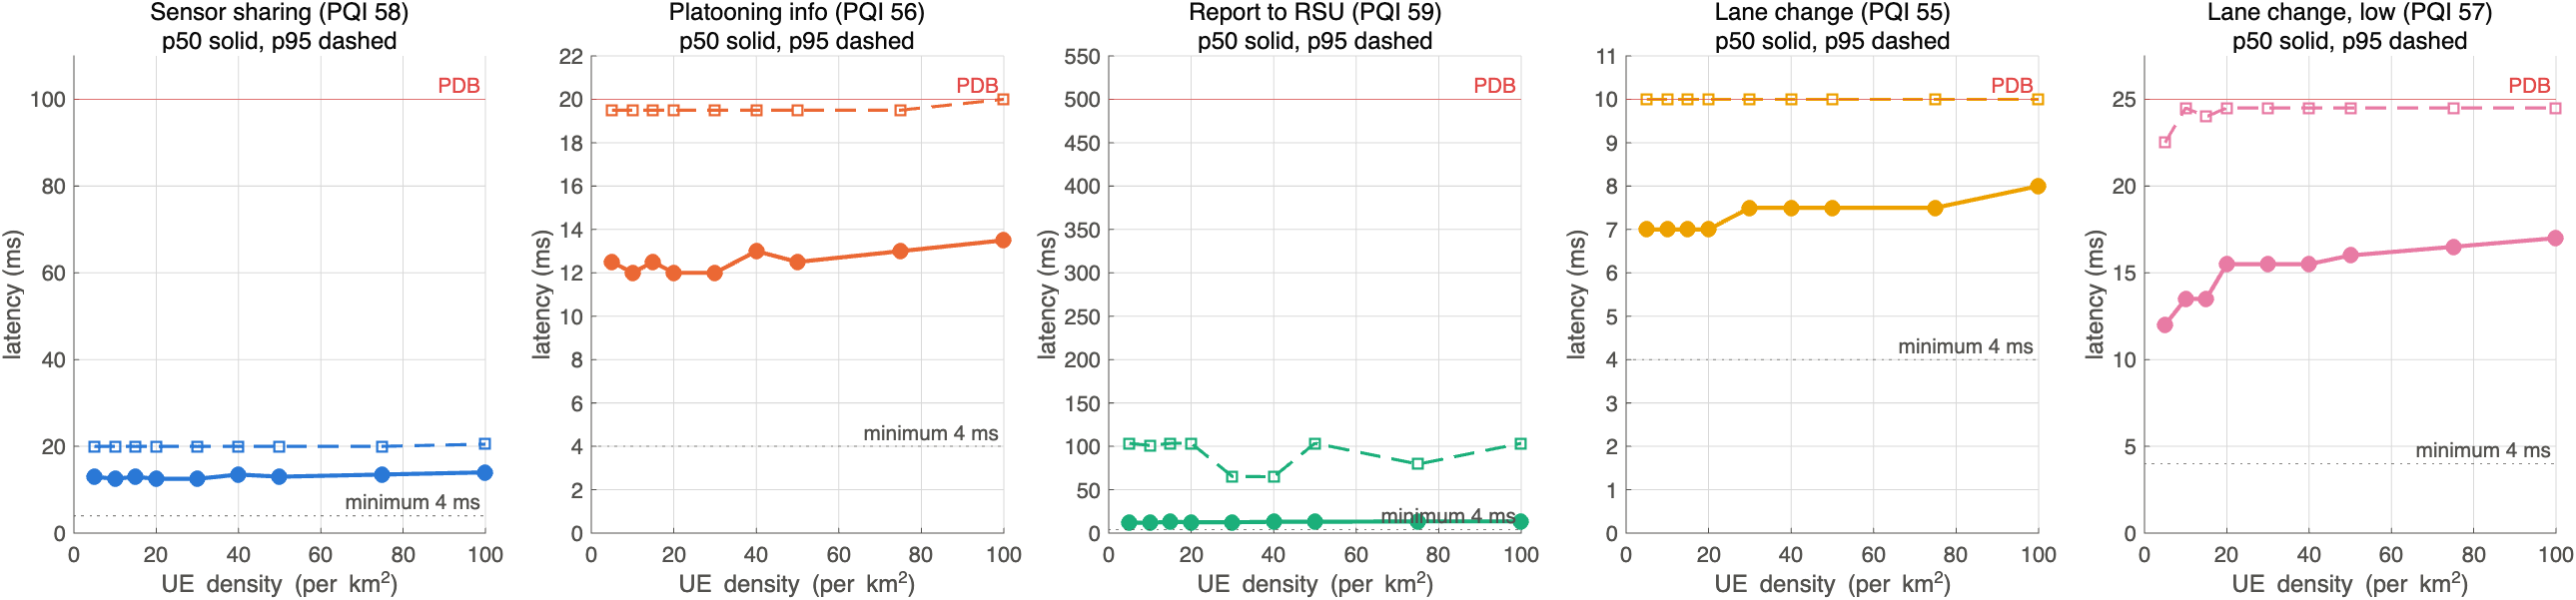
\includegraphics[width=\textwidth]{figures/C3_latency.png}
  \caption{Median (solid) and 95th-percentile (dashed) latency of
  delivered packets against density. Grey dotted: the 4~ms floor.}
  \label{fig:C3}
\end{figure}

\begin{table}[H]
\centering
\caption{System-level latency per flow, across densities.}
\label{tab:sllat}
\small
\begin{tabular}{c c c c}
\toprule
\textbf{Flow} & \textbf{PDB} & \textbf{Median} & \textbf{95th percentile} \\
\midrule
PQI 58 & 100~ms & 12.5--14~ms & 20--20.5~ms \\
PQI 56 & 20~ms  & 12--13.5~ms & 19.5--20~ms \\
PQI 59 & 500~ms & 12--13.5~ms & 65--104~ms \\
PQI 55 & 10~ms  & 7--8~ms     & 10~ms \\
PQI 57 & 25~ms  & 12--17~ms   & 22.5--24.5~ms \\
\bottomrule
\end{tabular}
\end{table}

\begin{itemize}[nosep]
  \item \textbf{Latency hardly changes with density.} Contention shows up
  as lost packets, not slower ones: a packet that collides on both
  transmissions is gone, not delivered late.
  \item \textbf{The long-PDB flows leave much earlier than their own
  window allows.} PQI~58's median is 13~ms against a 52~ms window mean
  (Table~\ref{tab:bounds}). These flows ride grants that the short-PDB
  flows keep reselecting with short windows.
  \item \textbf{Every flow's 95th percentile stays at or under its PDB},
  as the expiry rule guarantees.
\end{itemize}

\subsection{Throughput: What Broadcast Delivers with Sensing Running}
\label{sec:bcthr}

A broadcast transmission has many receivers, so its throughput is
counted where it is used, at the receivers:
\begin{itemize}[nosep]
  \item every copy of a packet that reaches an intended receiver (within
  500~m) within its PDB adds that packet's bits;
  \item \emph{ideal} is every intended receiver getting every packet;
  \item \emph{per UE} is the field total divided by the number of UEs:
  what an average UE receives on time.
\end{itemize}

\begin{figure}[H]
  \centering
  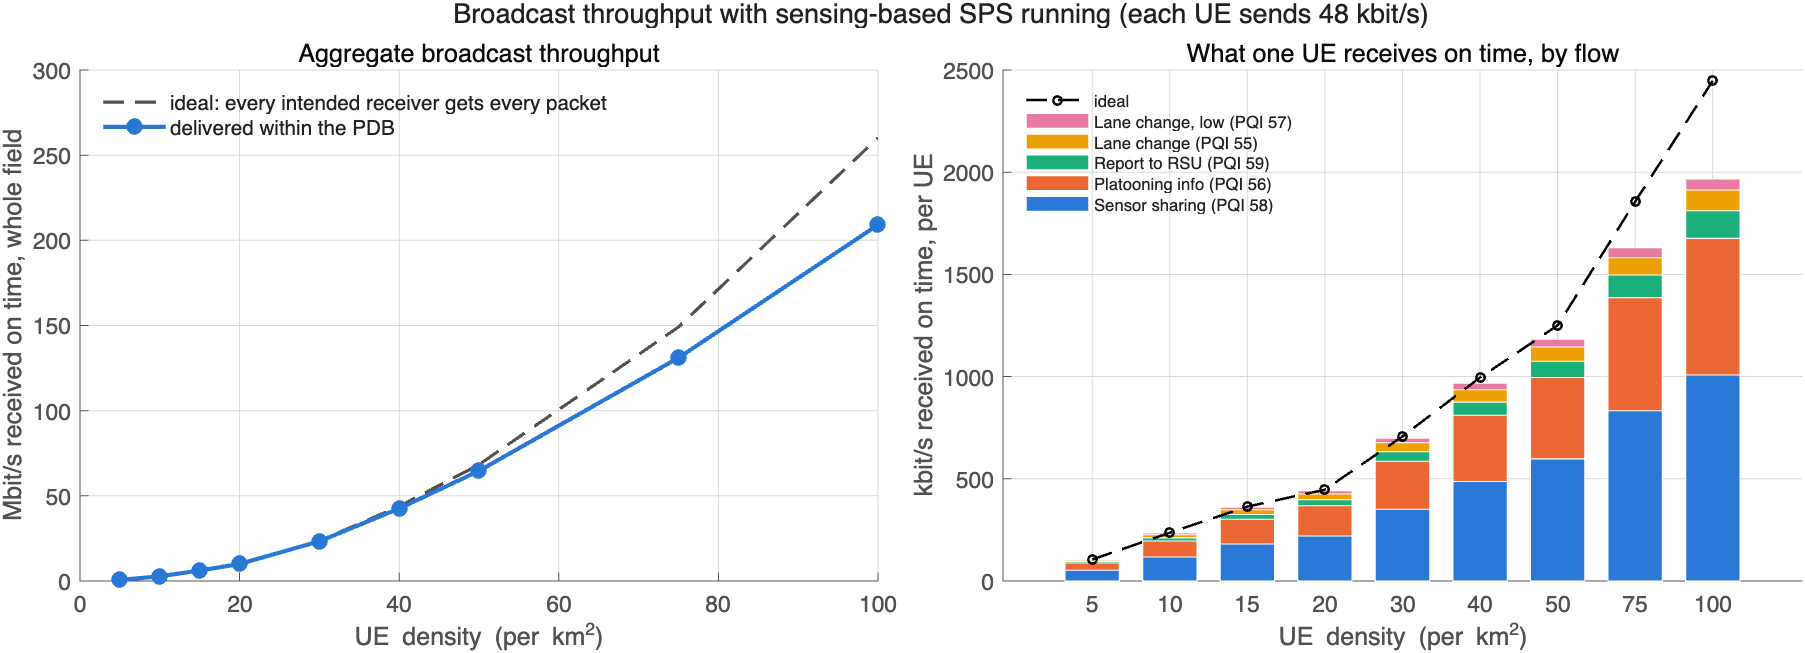
\includegraphics[width=\textwidth]{figures/C4_throughput.png}
  \caption{Broadcast throughput against density. Left: the whole field,
  delivered on time against ideal. Right: what one UE receives on time,
  split by flow; dashed: ideal.}
  \label{fig:C4}
\end{figure}

\begin{table}[H]
\centering
\caption{Broadcast throughput, counted at the receivers.}
\label{tab:bcthr}
\footnotesize\setlength{\tabcolsep}{3.5pt}
\begin{tabular}{r r r r r r}
\toprule
\textbf{Density} & \textbf{UEs} & \textbf{Ideal (field)} & \textbf{Delivered (field)} & \textbf{Received per UE} & \textbf{Efficiency} \\
\midrule
5   & 6   & 0.67~Mbit/s & 0.66~Mbit/s & 105~kbit/s  & 99.3\% \\
10  & 12  & 2.76~Mbit/s & 2.74~Mbit/s & 234~kbit/s  & 99.3\% \\
15  & 17  & 6.19~Mbit/s & 6.14~Mbit/s & 361~kbit/s  & 99.3\% \\
20  & 23  & 10.1~Mbit/s & 10.0~Mbit/s & 442~kbit/s  & 98.9\% \\
30  & 33  & 23.6~Mbit/s & 23.3~Mbit/s & 699~kbit/s  & 98.8\% \\
40  & 44  & 43.8~Mbit/s & 42.6~Mbit/s & 967~kbit/s  & 97.1\% \\
50  & 55  & 68.3~Mbit/s & 64.7~Mbit/s & 1183~kbit/s & 94.6\% \\
75  & 80  & 149~Mbit/s  & 131~Mbit/s  & 1631~kbit/s & 87.9\% \\
100 & 106 & 260~Mbit/s  & 209~Mbit/s  & 1967~kbit/s & 80.4\% \\
\bottomrule
\end{tabular}
\end{table}

\begin{itemize}[nosep]
  \item \textbf{Every UE transmits 48~kbit/s at every density}, and nearly
  all of it is sent. What changes is how many receivers get it in time.
  \item \textbf{Broadcast throughput grows with density, because every
  transmission is heard by more receivers.} One 48~kbit/s transmitter
  with 26 neighbours (50~UE/km$^2$) provides about 1.2~Mbit/s of useful
  reception.
  \item \textbf{Efficiency (delivered / ideal) is the cost of sharing.} It
  stays above 98.8\% up to 30~UE/km$^2$, then falls to 94.6\% at 50 and
  80.4\% at 100. At 100~UE/km$^2$ a fifth of the copies that should
  arrive are lost to collisions and half duplex.
  \item \textbf{Part~B's 14.3~Mbit/s for MCS~11 is one link holding the
  whole channel.} Here each UE uses about 0.3\% of that rate as a
  transmitter. The field is limited by collisions, not by link capacity.
\end{itemize}

\subsection{Collisions and Channel Load}
\label{sec:col}

\begin{figure}[H]
  \centering
  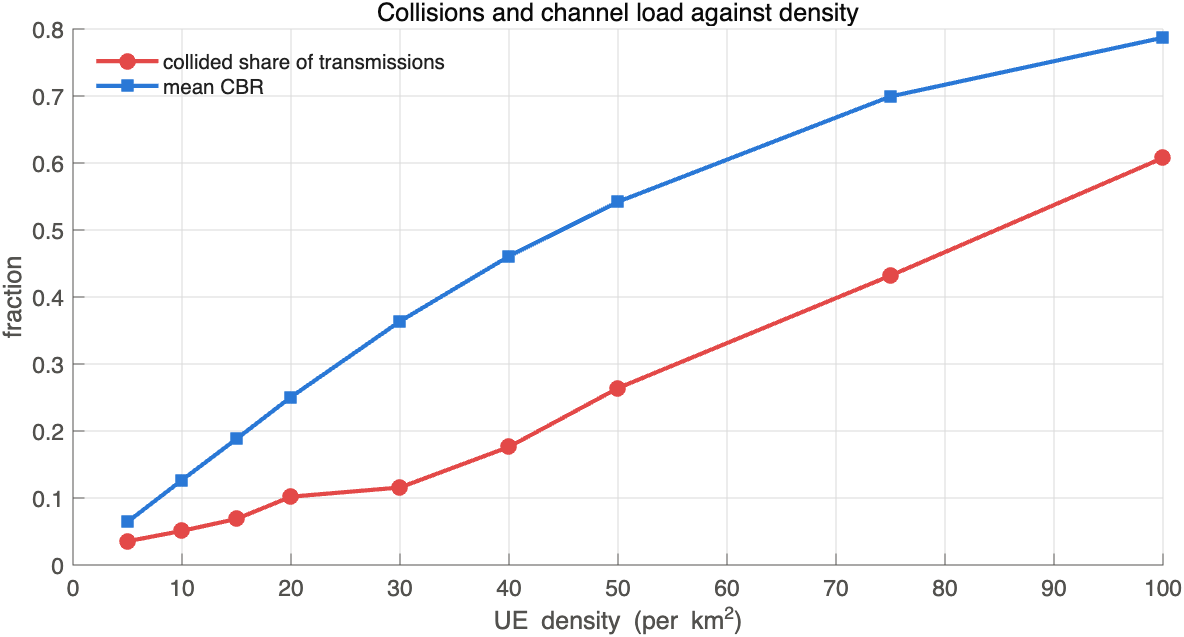
\includegraphics[width=0.85\textwidth]{figures/C5_collisions.png}
  \caption{Share of transmissions that collided, and mean channel busy
  ratio (CBR) \cite{ref:38215}.}
  \label{fig:C5}
\end{figure}

\begin{table}[H]
\centering
\caption{Collisions and channel busy ratio against density.}
\label{tab:col}
\small
\begin{tabular}{r c c}
\toprule
\textbf{Density (UE/km$^2$)} & \textbf{Collided transmissions} & \textbf{Mean CBR} \\
\midrule
5   & 3.5\%  & 0.06 \\
10  & 5.1\%  & 0.13 \\
15  & 6.9\%  & 0.19 \\
20  & 10.2\% & 0.25 \\
30  & 11.6\% & 0.36 \\
40  & 17.6\% & 0.46 \\
50  & 26.4\% & 0.54 \\
75  & 43.2\% & 0.70 \\
100 & 60.8\% & 0.79 \\
\bottomrule
\end{tabular}
\end{table}

A collision here means two transmissions in the same slot sharing at
least one sub-channel, anywhere in the field. Because every transmission
spans the full channel, any two in the same slot collide. Most are
between UEs far enough apart that each receiver still decodes the nearer
one. That is why 61\% collided transmissions turn into 18\% lost copies
for the periodic flows and 31--38\% for the events.

\subsection{Why Packets Fail}
\label{sec:fail}

\begin{figure}[H]
  \centering
  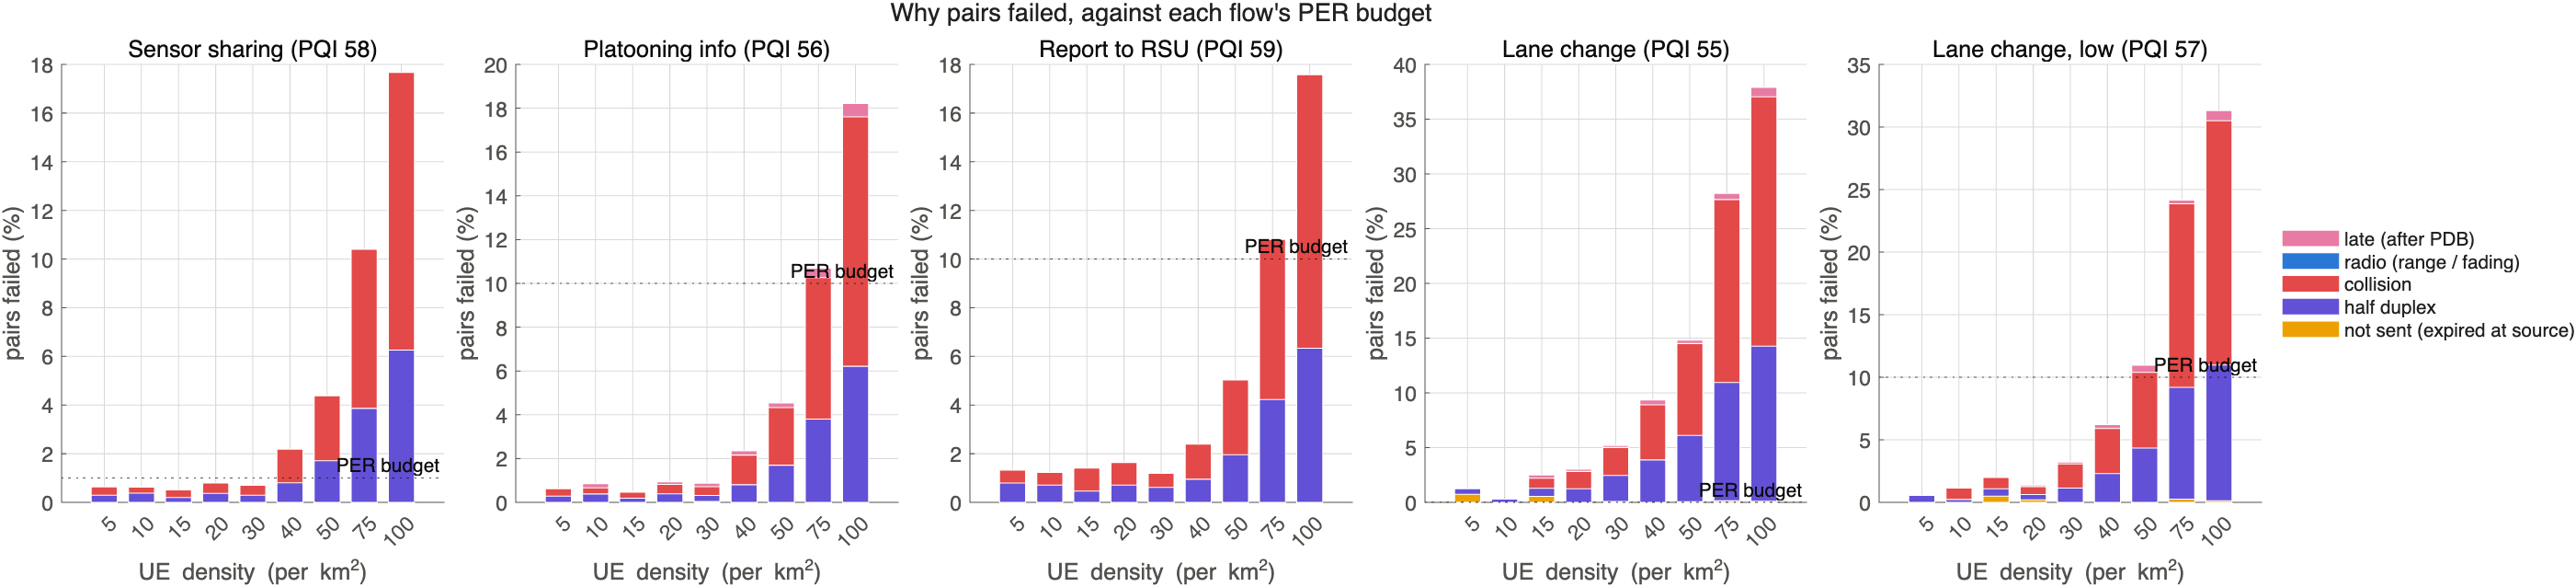
\includegraphics[width=\textwidth]{figures/C6_failures.png}
  \caption{Failed pairs by cause, against each flow's PER budget (dotted).}
  \label{fig:C6}
\end{figure}

\begin{table}[H]
\centering
\caption{Causes of failure.}
\label{tab:fail}
\small
\begin{tabularx}{\textwidth}{X l}
\toprule
\textbf{Cause} & \textbf{Share of failures} \\
\midrule
\textbf{Collision}: a transmission shared slot and sub-channel with another and was not decoded & 37--67\% (from 15~UE/km$^2$) \\
\textbf{Half duplex}: the receiver was itself transmitting in every slot the packet was sent & 30--60\% (from 15~UE/km$^2$) \\
Late: decoded only on a retransmission after the PDB & 0--22\% (mostly PQI 56) \\
Not sent: expired at the sender before a resource came up & under 1\% above 20~UE/km$^2$ \\
Radio: clean, but too far or faded & 0\% (receivers within 500~m) \\
\bottomrule
\end{tabularx}
\end{table}

\begin{itemize}[nosep]
  \item \textbf{Contention causes every loss.} The radio link is never
  the limit inside 500~m.
  \item \textbf{Half duplex and collisions are about equal} at every
  density. Each UE transmits often (five flows, about 6.5 reselections a
  second), and while it transmits it cannot hear.
\end{itemize}

\subsection{Reliability against Distance}
\label{sec:reldist}

\begin{figure}[H]
  \centering
  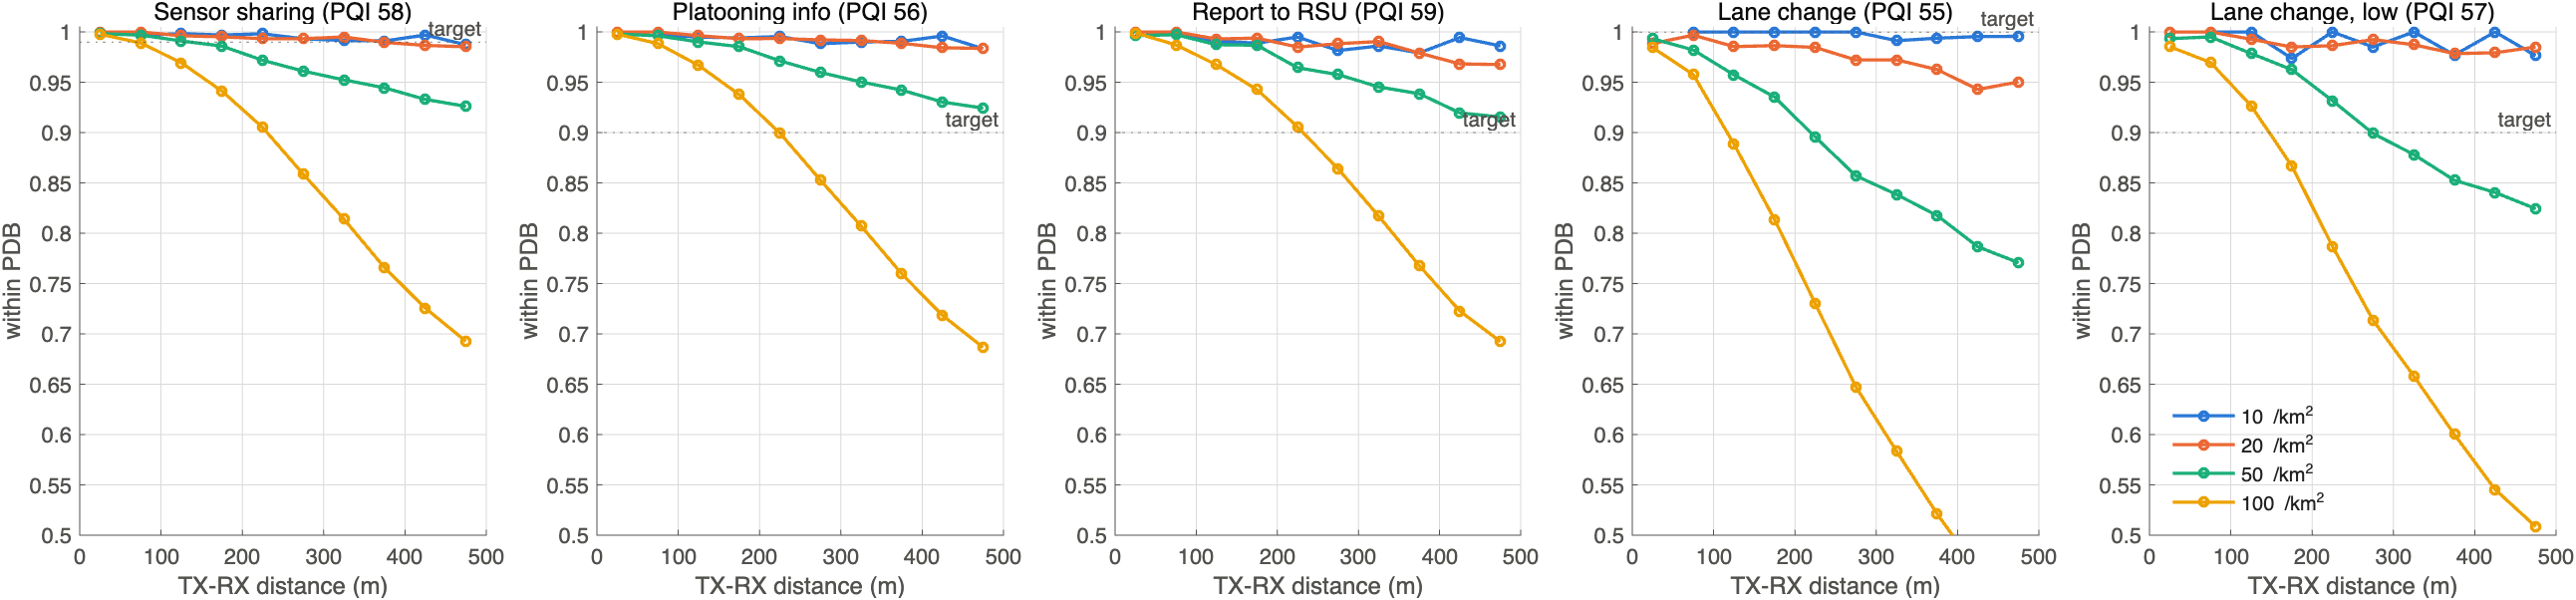
\includegraphics[width=\textwidth]{figures/C7_reliability_vs_distance.png}
  \caption{Share delivered within the PDB against sender--receiver
  distance, for 10, 20, 50 and 100~UE/km$^2$.}
  \label{fig:C7}
\end{figure}

\begin{itemize}[nosep]
  \item \textbf{Near the sender every flow is reliable at every density:}
  within about 50~m every flow delivers at least 98\%, because the
  sender is far louder than any interferer.
  \item \textbf{Reliability falls with distance}, because the further the
  receiver, the more interferers are as loud as the wanted signal.
\end{itemize}
The usable range of a flow in a crowded field is set by density, not by
the MCS.

\subsection{Part C Summary}

With every UE carrying all five broadcast PQIs at 48~kbit/s:
\begin{itemize}[nosep]
  \item the 90\% flows hold their targets up to about 70~UE/km$^2$
  (PQIs 56, 59) and 48~UE/km$^2$ (PQI~57);
  \item the 99\% sensor-sharing flow (PQI~58) holds to about
  32~UE/km$^2$;
  \item the 99.99\% lane-change flow (PQI~55) is not met at any density;
  \item broadcast throughput reaches every intended receiver with at
  least 98.8\% efficiency up to 30~UE/km$^2$ (23~Mbit/s of on-time
  reception in the field, about 0.7~Mbit/s per UE), falling to 80\% at
  100~UE/km$^2$;
  \item latency stays near the bottom of each window and does not grow
  with density: contention costs packets, not time;
  \item every loss is a collision or half duplex. Carrying five flows on
  one grant makes both worse: every transmission spans the whole 20~MHz,
  and the short-PDB flows reselect the grant about six times a second.
\end{itemize}
The levers for the 99\% and 99.99\% flows are therefore separate grants
per flow class, more retransmissions for the tight flows only,
congestion control (the \code{sl-CR-Limit} response to CBR), and more
spectrum.

%==========================================================================
\newpage
\section{Assumptions and Limits}
\label{sec:limits}

\begin{itemize}
  \item \textbf{Propagation is TR~38.901 RMa, line of sight}
  \cite{ref:38901}. RMa is specified for base-station heights of
  10--150~m; here both ends are at 3~m. That is outside its stated range,
  but it is the standard rural model and its two-slope shape (20 then
  40~dB per decade) is physical. There is no shadowing or obstruction:
  an open field.
  \item \textbf{Antenna height (3~m) and gain (3~dBi each) are deployment
  assumptions} for agricultural machinery. The noise figure (9~dB) is
  TR~37.885 V15.3.0 Table~6.1.1-1 \cite{ref:37885}.
  \item \textbf{Speed is the relative speed of the link} and enters
  through the Doppler of the fading channel.
  \item \textbf{Part~B latency has no other users}; contention appears
  only in Part~C.
  \item \textbf{One grant per UE in Part~C.} All of a UE's flows share one
  sidelink grant, sized for all of them. A real UE may run several (see
  Section~\ref{sec:traffic}).
  \item \textbf{Latency counts 3 slots from the transmission slot} (1 on
  the air, 2 to receive), and no packet is transmitted sooner than
  $\Tproc$ after it arrives.
  \item \textbf{Part~C's PHY is abstracted} through the BLER tables Part~B
  measured (at 20~mph), because a 1~km$^2$ field of up to 100 UEs cannot
  be simulated sample by sample in reasonable time. A separate
  waveform-level check of this abstraction found it accurate to about
  1~dB.
  \item \textbf{One known deviation from the specification is open:} the
  PSSCH resource mapping starts at the first DM-RS symbol rather than at
  \code{sl-StartSymbol} + 1 (TS~38.214 \S8.1.2.1) \cite{ref:38214}. It
  slightly understates the data capacity of wide allocations.
\end{itemize}

\section{Reproducing the Results}
\label{sec:repro}

All results are produced by the \code{experiments} package of the
\code{nrSidelink} repository:
\begin{center}
\small
\begin{tabular}{l l l}
\toprule
\textbf{Part} & \textbf{Function} & \textbf{Figures} \\
\midrule
A & \code{experiments.macTutorial} & \code{plots/study/A\_mac/} \\
B & \code{experiments.linkLevel} (BLER from \code{experiments.measureSpeeds}) & \code{plots/study/B\_link/} \\
C & \code{experiments.systemLevel}, \code{experiments.deployment} & \code{plots/study/C\_system/} \\
\bottomrule
\end{tabular}
\end{center}
\code{experiments.runStudy()} runs all three parts; the operating point
and the link (path loss, antenna height and gain, noise figure) are set
in \code{+experiments/settings.m}.

\section*{Glossary}
\addcontentsline{toc}{section}{Glossary}

\begin{table}[H]
\centering
\small
\begin{tabularx}{\textwidth}{l X}
\toprule
\textbf{Term} & \textbf{Meaning} \\
\midrule
Mode~2 & sidelink resource allocation where each UE selects its own resources \\
PDB / PER & packet delay budget / packet error rate allowed; a late packet counts as an error \\
PQI & PC5 QoS identifier: a row of TS~23.287 Table~5.4.4-1 fixing PDB, PER and priority \\
SCI-1A & first-stage control message; announces where the sender transmits and reserves \\
TRIV / FRIV & SCI fields giving the time / frequency of the chained retransmission \\
$\Lsub$ & number of sub-channels a transmission occupies \\
$S_A$ & candidate set after exclusion \\
$\Tone$, $\Ttwo$ & start and end of the selection window, in slots after the packet's arrival \\
SPS & semi-persistent scheduling: the same resource reused every reservation period \\
$\Prsvp$ & reservation period \\
RSRP & reference signal received power, per resource element \\
CBR & channel busy ratio: share of sub-channels sensed busy in the last 100~ms \\
MCS & modulation and coding scheme \\
BLER & block error rate: share of transport blocks failing LDPC decoding or the CRC \\
PPP & Poisson point process: random UE positions with a Poisson-distributed count \\
\bottomrule
\end{tabularx}
\end{table}

%==========================================================================
\begin{thebibliography}{99}
\addcontentsline{toc}{section}{References}

\bibitem{ref:38211} 3GPP TS 38.211 V16.10.0, \emph{NR; Physical channels and modulation (Release 16)}.
\bibitem{ref:38212} 3GPP TS 38.212 V16.15.0, \emph{NR; Multiplexing and channel coding (Release 16)}.
\bibitem{ref:38214} 3GPP TS 38.214 V16.17.0, \emph{NR; Physical layer procedures for data (Release 16)}.
\bibitem{ref:38215} 3GPP TS 38.215 V16.7.0, \emph{NR; Physical layer measurements (Release 16)}.
\bibitem{ref:38321} 3GPP TS 38.321 V16.22.0, \emph{NR; Medium Access Control (MAC) protocol specification (Release 16)}.
\bibitem{ref:23287} 3GPP TS 23.287 V19.0.0, \emph{Architecture enhancements for 5G System (5GS) to support Vehicle-to-Everything (V2X) services}.
\bibitem{ref:37885} 3GPP TR 37.885 V15.3.0, \emph{Study on evaluation methodology of new Vehicle-to-Everything (V2X) use cases for LTE and NR (Release 15)}.
\bibitem{ref:38901} 3GPP TR 38.901, \emph{Study on channel model for frequencies from 0.5 to 100 GHz}.

\end{thebibliography}

\end{document}
